\subsection{Set Representations} \label{sec:setRepresentations}
\logToConsole{SET REPRESENTATIONS}

The basis of any efficient reachability analysis is an appropriate set representation. On the one hand, the set representation should be general enough to describe the reachable sets accurately; on the other hand, it is crucial that the set representation facilitates efficient and scalable operations on them. CORA provides a wide range of set representations that are explained in detail in this section. \cref{tab:setConversion} shows the supported conversions between set representations. In order to convert a set, it is sufficient to pass the current set to the class constructor of the target set representation, as demonstrated by the following example:

    {\footnotesize % This file was automatically created from the m-file 
% "m2tex.m" written by USL. 
% The fontencoding in this file is UTF-8. 
%  
% You will need to include the following two packages in 
% your LaTeX-Main-File. 
%  
% \usepackage{color} 
% \usepackage{fancyvrb} 
%  
% It is advised to use the following option for Inputenc 
% \usepackage[utf8]{inputenc} 
%  
  
% definition of matlab colors: 
\definecolor{mblue}{rgb}{0,0,1} 
\definecolor{mgreen}{rgb}{0.13333,0.5451,0.13333} 
\definecolor{mred}{rgb}{0.62745,0.12549,0.94118} 
\definecolor{mgrey}{rgb}{0.5,0.5,0.5} 
\definecolor{mdarkgrey}{rgb}{0.25,0.25,0.25} 
  
\DefineShortVerb[fontfamily=courier,fontseries=m]{\$} 
\DefineShortVerb[fontfamily=courier,fontseries=b]{\#} 
  
\noindent      
 $  $\color{mgreen}$% create zonotope object$\color{black}$$\\
 $  Z = zonotope([1 2 1;0 1 -1]);$\\
 $  $\\
 $  $\color{mgreen}$% convert to other set representations$\color{black}$$\\
 $  I = interval(Z);           $\color{mgreen}$% over-approximative conversion to an interval$\color{black}$$\\
 $  P = polytope(Z);       $\color{mgreen}$% exact conversion to polytope$\color{black}$$\\
  
\UndefineShortVerb{\$} 
\UndefineShortVerb{\#}}

\begin{table}[htb]
    \centering
    \footnotesize
    \caption{Set conversions supported by CORA. The row headers represent the original set representation and the column headers the target set representation after conversion. The shortcuts e (exact conversion) and o (over-approximation) are used.}
    \label{tab:setConversion}
    \begin{tabular}{ l c c c c c c c c c c c}
        \toprule
        & \textbf{Z} & \textbf{zB} & \textbf{pZ} & \textbf{cPZ} & \textbf{cZ} & \textbf{P} & \textbf{I} & \textbf{tay} & \textbf{C} & \textbf{E} & \textbf{SpS}\\
        \midrule
        \textbf{zonotope} (Z, \cref{sec:zonotope})                       & -          & e           & e           & e            & e           & e          & o          & e            & o          & o          & e          \\
        \textbf{zonoBundle} (zB, \cref{sec:zonoBundle})                  & o          & -           & e           & e            & e           & e          & o          &              &            &            & e          \\
        \textbf{polyZonotope} (pZ, \cref{sec:polynomialZonotopes})       & o          &             & -           & e            &             & o          & o          & o            &            & o          & o          \\
        \textbf{conPolyZono} (cPZ, \cref{sec:conPolyZono})               & o          & o           & o           & -            & o           & o          & o          & o            & o          & o          &            \\
        \textbf{probZonotope} (probZ, \cref{sec:probabilisticZonotopes}) & o          &             &             &              &             &            &            &              &            &            &            \\
        \textbf{conZonotope} (cZ, \cref{sec:conZonotope})                & o          & e           & e           & e            & -           & e          & o          &              &            &            & e          \\
        \textbf{polytope} (P, \cref{sec:polytopes})                      &            & e           & e           & e            & e           & -          & o          &              &            &            & e          \\
        \textbf{interval} (I, \cref{sec:interval})                       & e          & e           & e           & e            & e           & e          & -          &              & o          & o          & e          \\
        \textbf{taylm} (tay, \cref{sec:taylorModels})                    &            &             &             & e            &             &            & o          & -            &            &            &            \\
        \textbf{capsule} (C, \cref{sec:capsules})                        & o          &             &             & e            &             &            & o          &              & -          &            & e          \\
        \textbf{ellipsoid} (E, \cref{sec:ellipsoids})                    & o          &             &             & e            &             &            & o          &              &            & -          & e          \\
        \textbf{spectraShadow} (SpS, \cref{sec:spectraShadow})    & o          & o           & o           & o            & o           &            & o          &              &            &            & -          \\
        \bottomrule
    \end{tabular}
\end{table}

% Basic set representations --------------------------------------------------------------------------------------------

\subsubsection{Basic Set Representations} \label{sec:basicSetRep}

We first introduce basic set representations predominantly used to represent reachable sets.

\subsubsubsection{Zonotopes} \label{sec:zonotope}

A zonotope $\mathcal{Z} \subset \mathbb{R}^n$ is defined as
\begin{equation} \label{eq:zonotope}
\mathcal{Z} := \bigg \{ c + \sum_{i=1}^{p} \beta_i g\^{i} ~\bigg|~ \beta_i \in [-1,1] \bigg\},
\end{equation}
where $c \in \mathbb{R}^n$ is the center and $g\^i \in \mathbb{R}^n$ are the generators. The zonotope order $\rho$ is defined as $\rho = \frac{p}{n}$ and represents a dimensionless measure for the representation size.

Zonotopes are represented in CORA by the class \texttt{zonotope}. An object of class \texttt{zonotope} can be constructed as follows:
\begin{equation*}
	\begin{split}
		& \mathcal{Z} = \texttt{zonotope}(c,G), \\
		& \mathcal{Z} = \texttt{zonotope}(Z),
	\end{split}
\end{equation*} 
where $G= [g^{(1)},\dots,g^{(p)}]$, $Z = [c,G]$, and $c,g^{(i)}$ are defined as in \eqref{eq:zonotope}. Let us demonstrate the construction of a zonotope by an example:

\begin{center}
\begin{minipage}[t]{0.35\textwidth}
	\vspace{20pt}
	\footnotesize
	\input{./MATLABcode/example_setRep_zonotope}
\end{minipage}
\begin{minipage}[t]{0.3\textwidth}
	\vspace{0pt}
	\centering
	\includetikz{./figures/tikz/set-representations/example_zonotope}
\end{minipage}
\end{center}

A more detailed example for zonotopes is provided in \cref{sec:zonotopeExample} and in the file \textit{examples/contSet/example\_zonotope.m} in the CORA toolbox.

A zonotope can be interpreted as the Minkowski addition of line segments $l\^i = [-1,1]g\^{i}$. The step-by-step construction of a two-dimesional zonotope is visualized in \cref{fig:zonotope}. Zonotopes are a compact representation of sets in high-dimensional space. More importantly, operations required for reachability analysis, such as linear maps (see \cref{sec:mtimes}) and Minkowski addition (see \cref{sec:plus}) can be computed efficiently and exactly, and others, such as convex hull computation (see \cref{sec:convHull}) can be tightly over-approximated \cite{Girard2005}.

\begin{figure}[htb]
	\centering
	\includetikz{./figures/tikz/set-representations/example_zonotope_construction}
	\caption{Step-by-step construction of a zonotope.}
	\label{fig:zonotope}
\end{figure}

In addition to the standard set operations described in \cref{sec:setOperations} and the methods for converting between set operations (see \cref{tab:setConversion}), the class \texttt{zonotope} supports additional methods which are listed in \cref{sec:zonotopeOperations}.

\subsubsubsection{Intervals} \label{sec:interval}

A real-valued multi-dimensional interval
\begin{equation}
	\mathcal{I} :=\{x \in \mathbb{R}^n ~|~ \underline{x}_i \leq x_i \leq \overline{x}_i ~\forall i = 1,\dots,n \}
	\label{eq:interval}
\end{equation} 
is a connected subset of $\mathbb{R}^n$ and can be specified by a lower bound $\underline{x}\in\mathbb{R}^n$ and upper bound $\overline{x}\in\mathbb{R}^n$.

Intervals are represented in CORA by the class \texttt{interval}. An object of class \texttt{interval} can be constructed as follows:
\begin{equation*}
	\begin{split}
		& \mathcal{I} = \texttt{interval}(\underline{x},\overline{x}) \\
	\end{split}
\end{equation*} 
where $\underline{x},\overline{x}$ are defined as in \eqref{eq:interval}. A detailed description of how intervals are treated in CORA can be found in \cite{Althoff2016a}. Let us demonstrate the construction of an interval by an example:

\begin{center}
\begin{minipage}[t]{0.35\textwidth}
	\vspace{30pt}
	\footnotesize
	\input{./MATLABcode/example_setRep_interval}
\end{minipage}
\begin{minipage}[t]{0.3\textwidth}
	\vspace{0pt}
	\centering
	\includetikz{./figures/tikz/set-representations/example_interval}
\end{minipage}
\end{center}

A more detailed example for intervals is provided in \cref{sec:intervalExample} and in the file \textit{examples/contSet/example\_interval.m} in the CORA toolbox. Intervals can also be used for range bounding as it described in \cref{sec:rangeBounding}. In addition to the standard set operations described in \cref{sec:setOperations} and the methods for converting between set operations (see \cref{tab:setConversion}), the class \texttt{interval} supports additional methods, which are listed in \cref{sec:intervalOperations}.




\subsubsubsection{Ellipsoids} \label{sec:ellipsoids}

An ellipsoid is a geometric object in $\mathbb{R}^n$. Ellipsoids are parameterized by a center $q \in \mathbb{R}^n$ and a positive semi-definite, symmetric shape matrix $Q\in \mathbb{R}^{n\times n}$ and defined as\footnote{\href{Ellipsoidal Toolbox (Technical Report)}{https://www2.eecs.berkeley.edu/Pubs/TechRpts/2006/EECS-2006-46.pdf},  Sec. 2.2.4}
\begin{equation} \label{eq:ellipsoid}
	\mathcal{E} := \Big\{x\in \mathbb{R}^n ~ \Big| ~ l^Tx \leq l^Tq + \sqrt{l^TQl}, \ \forall l \in \mathbb{R}^n \Big \}.
\end{equation}
If we assume $Q$ to be invertible (which holds true for non-degenerate ellipsoids), it can be equivalently defined as (see \cite[Definition 2.1.3]{Kurzhanskiy2006})
\begin{equation*}
	\mathcal{E} := \Big\{ x\in \mathbb{R}^n ~ \Big| ~ \left(x-q\right)^T Q^{-1}\left(x-q\right)\leq 1 \Big \}.
\end{equation*}
Ellipsoids have a compact representation increasing only with dimension. Linear maps (see \cref{sec:mtimes}) can be computed exactly and efficiently, Minkowski sum (see \cref{sec:plus}) and others can be tightly over-approximated.

Ellipsoids are represented in CORA by the class \texttt{ellipsoid}. An object of class \texttt{ellipsoid} can be constructed as follows:
\begin{equation*}
	\begin{split}
		& \mathcal{E} = \texttt{ellipsoid}(Q), \\
		& \mathcal{E} = \texttt{ellipsoid}(Q,q),
	\end{split}
\end{equation*} 
where $Q,q$ are defined as in \eqref{eq:ellipsoid}. Let us demonstrate the construction of an ellipsoid by an example:

\begin{center}
\begin{minipage}[t]{0.35\textwidth}
	\vspace{30pt}
	\footnotesize
	\input{./MATLABcode/example_setRep_ellipsoid}
\end{minipage}
\begin{minipage}[t]{0.3\textwidth}
	\vspace{0pt}
	\centering
	\includetikz{./figures/tikz/set-representations/example_ellipsoid}
\end{minipage}
\end{center}

A more detailed example for ellipsoids is provided in \cref{sec:ellipsoidExample} and in the file \textit{examples/contSet/example\_ellipsoid.m} in the CORA toolbox. In addition to the standard set operations described in \cref{sec:setOperations} and the methods for converting between set operations (see \cref{tab:setConversion}), the class \texttt{ellipsoid} supports additional methods, which are listed in \cref{sec:ellipsoidOperation}.

\textbf{Note:} While the MPT toolbox comes with the semi-definite program solver SeDuMi\footnote{\url{https://sedumi.ie.lehigh.edu/}}, it proves to be somewhat unreliable for higher-dimensional systems. Therefore, we encourage users to install SDPT3\footnote{\url{https://www.math.cmu.edu/~reha/sdpt3.html}} as some operations on higher-dimensional ellipsoids will fail using SeDuMi.


\subsubsubsection{Polytopes} \label{sec:polytopes}

There exist two representations for polytopes: The halfspace representation (H-representation) and the vertex representation (V-representation).
Details of the implemented functionalities can be found in~\cite{Wetzlinger2024a}.

\paragraph{H-Representation of a Polytope}
The halfspace representation specifies a convex polytope $\mathcal{P}$ by the intersection of $q$ halfspaces $\mathcal{H}\^{i}$: $\mathcal{P}=\mathcal{H}\^{1} \cap \mathcal{H}\^{i} \cap \ldots \cap \mathcal{H}\^{q}$. A halfspace is one of the two parts obtained by bisecting the $n$-dimensional Euclidean space with a hyperplane $\mathcal{S}:=\{x \, | \, a^T x = b\}, a \in\mathbb{R}^{n},b\in\mathbb{R}$. The vector $a$ is the normal vector of the hyperplane and $b$ is the scalar product of any point on the hyperplane with the normal vector. From this follows that the corresponding halfspace is $\mathcal{H}:=\{x \, | \, a^T x\leq b\}$. As the convex polytope $\mathcal{P}$ is the non-empty intersection of $q$~halfspaces, all $q$~inequalities have to be fulfilled simultaneously.

A convex polytope $\mathcal{P}$ is the bounded intersection of $q$ halfspaces:
\begin{equation}
  \mathcal{P}:=\Big\{x \in \mathbb{R}^n ~\big|~ A\, x\leq b \Big\}, \quad A\in\mathbb{R}^{q\times n}, b\in\mathbb{R}^{q}.
  \label{eq:polytopeHalfspace}
\end{equation}
When the intersection is unbounded, one obtains a polyhedron \cite{Ziegler1995}.

\paragraph{V-Representation of a Polytope}
A polytope with vertex representation is defined as the convex hull of a finite set of points in the $n$-dimensional Euclidean space. The points are also referred to as vertices and denoted by $\mathtt{v}\^i\in\mathbb{R}^n$. A convex hull of a finite set of $r$ points $\mathtt{v}\^i\in\mathbb{R}^n$ is obtained from their linear combination:
\begin{equation}
\mathtt{Conv}(\mathtt{v}\^1,\ldots,\mathtt{v}\^r):=\Big\{\sum_{i=1}^{r} \alpha_i \mathtt{v}\^i ~\big|~ \alpha_i \in\mathbb{R}, \, \alpha_i\geq 0, \, \sum_{i=1}^{r} \alpha_i=1 \Big\}.
	\label{eq:polytopeVertex}
\end{equation}
%Given the convex hull operator $\mathtt{Conv}()$, a convex and bounded polytope can be defined in vertex representation as follows:


The halfspace and the vertex representation are illustrated in \cref{fig_polytope}. Algorithms that convert from H- to V-representation and vice versa are presented in \cite{Kaibel2003}.

\begin{figure}[htb]		
    \centering
	\subfigure[$V-representation$]{\includetikz{./figures/tikz/set-representations/polytope-v-representation}}
	\hspace{1cm}
	\subfigure[$H-representation$]{\includetikz{./figures/tikz/set-representations/polytope-h-representation}\label{fig:polytopeHRepresentation}}
	  \caption{Possible representations of a polytope.}
	  \label{fig_polytope}
\end{figure}


Polytopes are represented in CORA by the class \texttt{polytope}.
An object of class \texttt{polytope} can be constructed as follows:
\begin{equation*}
	\begin{split}
		& \mathcal{P} = \texttt{polytope}(V), \\
		& \mathcal{P} = \texttt{polytope}(A,b), \\
		& \mathcal{P} = \texttt{polytope}(A,b,Ae,be),
	\end{split}
\end{equation*} 
where $V = [v^{(1)},\dots,v^{(r)}]$, $v^{(i)}$ is defined as in \eqref{eq:polytopeVertex}, $A,b$ are defined as in \eqref{eq:polytopeHalfspace}, and $Ae,be$ are equality constraints that are used to compactly represent pairwise inequality constraints $a^\top x \leq b, a^\top x \geq b$. Let us demonstrate the construction of a polytope by an example:

\begin{center}
\begin{minipage}[t]{0.55\textwidth}
	\vspace{5pt}
	\footnotesize
	% This file was automatically created from the m-file 
% "m2tex.m" written by USL. 
% The fontencoding in this file is UTF-8. 
%  
% You will need to include the following two packages in 
% your LaTeX-Main-File. 
%  
% \usepackage{color} 
% \usepackage{fancyvrb} 
%  
% It is advised to use the following option for Inputenc 
% \usepackage[utf8]{inputenc} 
%  
  
% definition of matlab colors: 
\definecolor{mblue}{rgb}{0,0,1} 
\definecolor{mgreen}{rgb}{0.13333,0.5451,0.13333} 
\definecolor{mred}{rgb}{0.62745,0.12549,0.94118} 
\definecolor{mgrey}{rgb}{0.5,0.5,0.5} 
\definecolor{mdarkgrey}{rgb}{0.25,0.25,0.25} 
  
\DefineShortVerb[fontfamily=courier,fontseries=m]{\$} 
\DefineShortVerb[fontfamily=courier,fontseries=b]{\#} 
  
\noindent          
 $$\color{mgreen}$% construct polytope (halfspace rep.)$\color{black}$$\\
 $ A = [1 0 -1 0 1; 0 1 0 -1 1]';$\\
 $ b = [3; 2; 3; 2; 1];$\\
 $     $\\
 $ poly = polytope(A,b);$\\
 $ $\\
 $ $\color{mgreen}$% construct polytope (vertex rep.)$\color{black}$$\\
 $ V = [-3 -3 -1 3; -2 2 2 -2];$\\
 $ $\\
 $ poly = polytope(V);$\\
  
\UndefineShortVerb{\$} 
\UndefineShortVerb{\#}
\end{minipage}
\begin{minipage}[t]{0.3\textwidth}
	\vspace{0pt}
	\centering
	\includetikz{./figures/tikz/set-representations/example_polytope}
\end{minipage}
\end{center}

A more detailed example for polytopes is provided in \cref{sec:polytopeExample} and in the file \textit{examples/contSet/example\_polytope.m} in the CORA toolbox. In addition to the standard set operations described in \cref{sec:setOperations} and the methods for converting between set operations (see \cref{tab:setConversion}), the class \texttt{polytope} supports additional methods, which are listed in \cref{sec:polytopeOperations}.

\subsubsubsection{Polynomial Zonotopes} \label{sec:polynomialZonotopes}

Polynomial zonotopes, which were first introduced in \cite{Althoff2013a}, are a non-convex set representation. In CORA we implemented the sparse representation of polynomial zonotopes described in \cite{Kochdumper2021a}. A polynomial zonotope $\mathcal{PZ} \subset \Rn$ is defined as
\begin{equation}
    \mathcal{PZ} := \bigg\{ c + \sum _{i=1}^h \bigg( \prod _{k=1}^p \alpha _k ^{E_{(k,i)}} \bigg) G_{(\cdot,i)} + \sum _{j=1}^{q} \beta _j G_{I(\cdot,j)} ~ \bigg| ~ \alpha_k, \beta_j \in [-1,1] \bigg\},
  \label{eq:polyZonotope}
\end{equation}
where $c \in \Rn$ is the center, $G \in \mathbb{R}^{n \times h}$ the matrix of dependent generators, $G_I \in \mathbb{R}^{n \times q}$ the matrix of independent generators, and  $E \in \mathbb{N}_{0}^{p \times h}$ the exponent matrix. Since polynomial zonotopes can represent non-convex sets, and since they are closed under quadratic and higher-order maps, they are a good choice for reachability analysis.

Polynomial zonotopes are represented in CORA by the class \texttt{polyZonotope}. An object of class \texttt{polyZonotope} can be constructed as follows:
\begin{equation*}
	\begin{split}
	& \mathcal{PZ} = \texttt{polyZonotope}(c,G,G_I,E), \\
	& \mathcal{PZ} = \texttt{polyZonotope}(c,G,G_I,E,id), \\
	\end{split}
\end{equation*} 
where $c,G,G_I,E$ are defined as in \eqref{eq:polyZonotope}. The vector $id \in \mathbb{N}^p_{> 0}$ stores unambiguous identifiers for the dependent factors $\alpha_k$, which is important for dependency preservation as described in \cite{Kochdumper2020c}. Let us demonstrate the construction of a polynomial zonotope by an example:

\begin{center}
\begin{minipage}[t]{0.55\textwidth}
	\vspace{10pt}
	\footnotesize
	\input{./MATLABcode/example_setRep_polyZonotope}
\end{minipage}
\begin{minipage}[t]{0.3\textwidth}
	\vspace{0pt}
	\centering
	\includetikz{./figures/tikz/set-representations/example_polyZonotope}
\end{minipage}
\end{center}

This example defines the polynomial zonotope
\begin{equation*}
	\mathcal{PZ} = \bigg \{ \begin{bmatrix} 4 \\ 4 \end{bmatrix} + \alpha_1 \begin{bmatrix} 2 \\ 0 \end{bmatrix} + \alpha_2 \begin{bmatrix} 1 \\ 2 \end{bmatrix} + \alpha_1^3 \alpha_2 \begin{bmatrix} 2 \\ 2 \end{bmatrix} + \beta_1\begin{bmatrix} 1 \\ 0 \end{bmatrix}~\bigg|~ \alpha_1,\alpha_2,\beta_1 \in [-1,1] \bigg \}.
\end{equation*}
The construction of this polynomial zonotope is visualized in \cref{fig:polyZonotope}: (a) shows the set spanned by the constant offset vector and the first and second dependent generator, (b) shows the addition of the dependent generator with the mixed term $\alpha_1^3 \alpha_2$, (c) shows the addition of the independent generator, and (d) visualizes the final set.

\begin{figure}[htb]	
	\begin{center}
	\includetikz{./figures/tikz/set-representations/example_manual_polyZonotope_construction}
	\caption{Step-by-step construction of a polynomial zonotope.}
	\label{fig:polyZonotope}
	\end{center}
\end{figure}

A more detailed example for polynomial zonotopes is provided in \cref{sec:polyZonotopeExample} and in the file \textit{examples/contSet/example\_polyZonotope.m} in the CORA toolbox.

\subsubsubsection{Constrained Polynomial Zonotopes} \label{sec:conPolyZono}

Constrained polynomial zonotopes as introduced in \cite{Kochdumper2021c} extend the polynomial zonotopes in \cref{sec:polynomialZonotopes} by polynomial equality constraints on the dependent factors. Since constrained zonotopes are closed under all relevant set operations including intersection and union (see \cref{tab:basicOperations}), they are advantageous for many set-based algorithms. Furthermore, as shown in \cref{tab:setConversion}, most other set representations can be equivalently represented as constrained polynomial zonotopes, which further substantiates their importance. A constrained polynomial zonotope $\mathcal{CPZ} \subset \Rn$ is defined as
\begin{equation}
	\begin{split}
    \mathcal{CPZ} := \bigg\{ & c + \sum _{i=1}^h \bigg( \prod _{k=1}^p \alpha _k ^{E_{(k,i)}} \bigg) G_{(\cdot,i)} + \sum _{j=1}^{d} \beta _j G_{I(\cdot,j)} ~ \bigg| \\
    &  \sum _{i=1}^q \bigg( \prod _{k=1}^p \alpha _k ^{R_{(k,i)}} \bigg) A_{(\cdot,i)} = b, ~\alpha_k, \beta_j \in [-1,1] \bigg\},
    \end{split}
  \label{eq:conPolyZono}
\end{equation}
where $c \in \Rn$ is the constant offset, $G \in \mathbb{R}^{n \times h}$ the matrix of dependent generators, $G_I \in \mathbb{R}^{n \times d}$ the matrix of independent generators,  $E \in \mathbb{N}_{0}^{p \times h}$ the exponent matrix, $A \in \R^{m \times q}$ is the matrix of constraint generators, $b \in \R^m$ is the constraint offset, and $R \in \mathbb{N}_{0}^{p \times q}$ is the constraint exponent matrix. 

Constrained polynomial zonotopes are represented in CORA by the class \texttt{conPolyZono}. An object of class \texttt{conPolyZono} can be constructed as follows:
\begin{equation*}
\begin{split}
	& \mathcal{CPZ} = \texttt{conPolyZono}(c,G,E), \\
    & \mathcal{CPZ} = \texttt{conPolyZono}(c,G,E,G_I), \\
    & \mathcal{CPZ} = \texttt{conPolyZono}(c,G,E,G_I,id), \\
    & \mathcal{CPZ} = \texttt{conPolyZono}(c,G,E,A,b,R), \\
    & \mathcal{CPZ} = \texttt{conPolyZono}(c,G,E,A,b,R,G_I), \\
    & \mathcal{CPZ} = \texttt{conPolyZono}(c,G,E,A,b,R,G_I,id),
\end{split}
\end{equation*} 
where $c,G,G_I,E,A,b,R$ are defined as in \eqref{eq:conPolyZono}. The vector $id \in \mathbb{N}^p_{> 0}$ stores unambiguous identifiers for the dependent factors $\alpha_k$, which is important for dependency preservation as described in \cite{Kochdumper2020c}. Let us demonstrate constrained polynomial zonotopes with an example:

\begin{center}
\begin{minipage}[t]{0.55\textwidth}
	\vspace{10pt}
	\footnotesize
	\input{./MATLABcode/example_setRep_conPolyZono}
\end{minipage}
\begin{minipage}[t]{0.3\textwidth}
	\vspace{0pt}
	\centering
	\includetikz{./figures/tikz/set-representations/example_conPolyZono}
\end{minipage}
\end{center}

This example defines the constrained polynomial zonotope
\begin{equation*}
\begin{split}
		\mathcal{CPZ} = \bigg \{ & \begin{bmatrix} 0 \\ 0 \end{bmatrix} + \begin{bmatrix} 1 \\ 0 \end{bmatrix} \alpha_1 + \begin{bmatrix} 0 \\ 1 \end{bmatrix} \alpha_2 + \begin{bmatrix} 1 \\ 1 \end{bmatrix} \alpha_1 \alpha_2 \alpha_3 + \begin{bmatrix} -1 \\ 1 \end{bmatrix} \alpha_1^2 \alpha_3 ~ \bigg |  \\
		& ~ \alpha_2 - 0.5 \alpha_1 \alpha_3 + 0.5 \alpha_1^2 = 0.5, ~ \alpha_1,\alpha_2,\alpha_3 \in [-1,1] \bigg \}.
	\end{split}
\end{equation*}

A more detailed example for constrained polynomial zonotopes is provided in \cref{sec:conPolyZonoExample} and in the file \textit{examples/contSet/example\_conPolyZono.m} in the CORA toolbox.

\subsubsubsection{Capsules} \label{sec:capsules}

A capsule $\mathcal{C} \subset \Rn$ is defined as the Minkowski sum (see \cref{sec:plus}) of a line segment $\mathcal{L}$ and a sphere $\mathcal{S}$:
\begin{equation} \label{eq:capsule}
	\mathcal{C} := \mathcal{L} \oplus \mathcal{S}, ~~ \mathcal{L} = \{c + g \alpha~|~ \alpha \in [-1,1]\}, ~ \mathcal{S} = \{ x~|~ ||x||_2 \leq r \},
\end{equation}
where $c,g \in \Rn$ represent the center and the generator of the line segment, respectively, and $r \in \mathbb{R}_{\geq 0}$ is the radius of the sphere.

Capsules are represented in CORA by the class \texttt{capsule}. An object of class \texttt{capsule} can be constructed as follows:
\begin{equation*}
	\begin{split}
		& \mathcal{C} = \texttt{capsule}(c), \\
		& \mathcal{C} = \texttt{capsule}(c,g), \\
		& \mathcal{C} = \texttt{capsule}(c,r), \\
		& \mathcal{C} = \texttt{capsule}(c,g,r), \\
	\end{split}
\end{equation*} 
where $c,g,r$ are defined as in \eqref{eq:capsule}. Let us demonstrate the construction of a capsule by an example:

\begin{center}
\begin{minipage}[t]{0.35\textwidth}
	\vspace{30pt}
	\footnotesize
	\input{./MATLABcode/example_setRep_capsule}
\end{minipage}
\begin{minipage}[t]{0.3\textwidth}
	\vspace{0pt}
	\centering
	\includetikz{./figures/tikz/set-representations/example_capsule}
\end{minipage}
\end{center}

A more detailed example for capsules is provided in \cref{sec:capsuleExample} and in the file \textit{examples/contSet/example\_capsule.m} in the CORA toolbox.

\subsubsubsection{Zonotope Bundles} \label{sec:zonoBundle}

\normalsize
A disadvantage of zonotopes is that they are not closed under intersection, i.e., the intersection of two zonotopes does not return a zonotope in general. In order to overcome this disadvantage, zonotope bundles are introduced in \cite{Althoff2011f}. Given a finite set of zonotopes $\mathcal{Z}_i \subset \Rn$, a zonotope bundle is defined as 
\begin{equation} 
\mathcal{ZB} := \bigcap_{i=1}^{s} \mathcal{Z}_i,
\end{equation}
i.e., the intersection of the zonotopes $\mathcal{Z}_i$. Note that the intersection is not computed, but the zonotopes $\mathcal{Z}_i$ are stored in a list, which we write as $\mathcal{ZB} = \{ \mathcal{Z}_1, \ldots, \mathcal{Z}_s\}$.

Zonotope bundles are represented in CORA by the class \texttt{zonoBundle}. An object of class \texttt{zonoBundle} can be constructed as follows:
\begin{equation*}
	\begin{split}
		& \mathcal{ZB} = \texttt{zonoBundle}(\{ \mathcal{Z}_1, \ldots, \mathcal{Z}_s\}),
	\end{split}
\end{equation*} 
where the list of zonotopes $\{ \mathcal{Z}_1, \ldots, \mathcal{Z}_s\}$ is represented as a MATLAB cell array. Let us demonstrate the construction of a \texttt{zonoBundle} object by an example:

\begin{center}
\begin{minipage}[t]{0.5\textwidth}
	\vspace{15pt}
	\footnotesize
	\input{./MATLABcode/example_setRep_zonoBundle}
\end{minipage}
\begin{minipage}[t]{0.3\textwidth}
	\vspace{0pt}
	\centering
	\includetikz{./figures/tikz/set-representations/example_zonoBundle}
\end{minipage}
\end{center} 

A more detailed example for zonotope bundles is provided in \cref{sec:zonoBundleExample} and in the file \textit{examples/contSet/example\_zonoBundle.m} in the CORA toolbox. In addition to the standard set operations described in \cref{sec:setOperations} and the methods for converting between set operations (see \cref{tab:setConversion}), the class \texttt{zonoBundle} supports additional methods, which are listed in \cref{sec:zonoBundleOperations}.


\subsubsubsection{Constrained Zonotopes} \label{sec:conZonotope}

An extension of zonotopes described in \cref{sec:zonotope} are constrained zonotopes, which are introduced in \cite{Scott2016}. A constrained zonotope is defined as a zonotope with additional equality constraints on the factors $\beta_i$:
\begin{equation} \label{eq:constrainedZonotope}
	\mathcal{Z}_c := \Big\{ c + G \beta ~\Big|~ \lVert \beta \rVert_{\infty} \leq 1, A \beta = b \Big\}, 
\end{equation}
where $c \in \mathbb{R}^n$ is the zonotope center, $G \in \mathbb{R}^{n \times p}$ is the zonotope generator matrix and $\beta \in \mathbb{R}^p$ is the vector of zonotope factors. The equality constraints are parametrized by the matrix $A \in \mathbb{R}^{q \times p}$ and the vector $b \in \mathbb{R}^q$. Constrained zonotopes are able to describe arbitrary polytopes, and are therefore a more general set representation than zonotopes. The main advantage compared to a polytope representation using inequality constraints (see \cref{sec:polytopes}) is that constrained zonotopes inherit the excellent scaling properties of zonotopes for increasing state-space dimensions, since constrained zonotopes are also based on a generator representation for sets.

Constrained zonotopes are represented in CORA by the class \texttt{conZonotope}. An object of class \texttt{conZonotope} can be constructed as follows:
\begin{equation*}
	\begin{split}
		& \mathcal{Z}_c = \texttt{conZonotope}(c,G,A,b), \\
		& \mathcal{Z}_c = \texttt{conZonotope}(Z,A,b),
	\end{split}
\end{equation*} 
where $Z = [c,G]$, and $c,G,A,b$ are defined as in \eqref{eq:constrainedZonotope}. Let us demonstrate the construction of a constrained zonotope by an example:

\begin{center}
\begin{minipage}[t]{0.5\textwidth}
	\vspace{20pt}
	\footnotesize
	\input{./MATLABcode/example_setRep_conZonotope}
\end{minipage}
\begin{minipage}[t]{0.3\textwidth}
    \vspace{0pt}
    \centering
    \includetikz{./figures/tikz/set-representations/example_conZonotope}
\end{minipage}
\end{center}

The unconstrained zonotope from this example is visualized in \cref{fig:conZonotope1}, and the equality constraints in \cref{fig:conZonotope2}.

\begin{figure}[h!tb]
\begin{minipage}{0.45\columnwidth}
  \centering
  %\footnotesize
  \includetikz{./figures/tikz/set-representations/example_conZonotope_zonotope}
  \caption{Zonotope (red) and the corresponding constrained zonotope (blue).}
  \label{fig:conZonotope1}
\end{minipage}
\hspace{0.08\columnwidth}
\begin{minipage}{0.45\columnwidth}
  \centering
  %\footnotesize
  \includetikz{./figures/tikz/set-representations/example_conZonotope_constraints}
  \caption{Visualization of the equality constraints of the constrained zonotope.}
  \label{fig:conZonotope2}
\end{minipage}
\end{figure}

A more detailed example for constrained zonotopes is provided in \cref{sec:conZonotopeExample} and in the file \textit{examples/contSet/example\_conZonotope.m} in the CORA toolbox. In addition to the standard set operations described in \cref{sec:setOperations} and the methods for converting between set operations (see \cref{tab:setConversion}), the class \texttt{conZonotope} supports additional methods, which are listed in \cref{sec:conZonotopeOperations}.

\subsubsubsection{Spectrahedral Shadows} \label{sec:spectraShadow}

Spectrahedral shadows can be seen as the semidefinite generalization of polytopes, and can represent a large variety of convex sets. In particular, every convex set representation (e.g., zonotopes, intervals, ellipsoids, polytopes, capsules, zonotope bundles, and constrained zonotopes) implemented in CORA can be represented as a spectrahedral shadow. Formally, a spectrahedral shadow $\mathcal{SPS} \subseteq \Rn$ is defined as
\begin{equation} \label{eq:spectrahedralShadow}
	\mathcal{SPS} := \bigg \{ c + \sum_{i=1}^{p} \beta_i g\^{i} ~\bigg|~ A_{(0)} + \sum_{i=1}^p \beta_i A_{(i)} \succeq 0 \bigg\},
\end{equation}
where $c \in \mathbb{R}^n$ is the center vector, $g\^i \in \mathbb{R}^n$ are the generators, $A_{(i)}$ are symmetric coefficient matrices, and for a matrix $M$ the expression $M \succeq 0$ means that $M$ is positive semidefinite. If the matrix $G$ with columns $g\^i$ is the identity matrix, then $\mathcal{SPS}$ is also called a spectrahedron.

As shown in \cite[Lemma 4.1.5.]{Netzer2011}, non-empty spectrahedral shadows can equivalently be defined as
\begin{equation} \label{eq:spectrahedralShadow_existentialSum}
	\mathcal{SPS} := \bigg \{ x \in \Rn ~\bigg|~ \exists y \in \mathbb{R}^q, A_{(0)} + \sum_{i=1}^p x_i A_{(i)} + \sum_{j=1}^q y_j B_{(j)} \succeq 0 \bigg\},
\end{equation}
where $A_{(i)}$ and $B_{(j)}$ are symmetric coefficient matrices. We call this representation the existential sum representation.

Spectrahedral shadows are represented in CORA by the class \texttt{spectraShadow}. An object of class \texttt{spectraShadow} can be constructed as follows:
\begin{equation*}
	\begin{split}
		& \mathcal{SPS} = \texttt{spectraShadow}(A), \\
		& \mathcal{SPS} = \texttt{spectraShadow}(A,c), \\
		& \mathcal{SPS} = \texttt{spectraShadow}(A,c,G), \\
		& \mathcal{SPS} = \texttt{spectraShadow}(E), \\
	\end{split}
\end{equation*} 
where $G= [g^{(1)},\dots,g^{(p)}]$, with $c, g^{(i)}$ defined as in \eqref{eq:spectrahedralShadow} (if they are not specified, $c$ is chosen to be the origin, and $G$ the identity matrix). The matrix $A$ is the horizontal concatenation of the coefficient matrices $A_{(0)},\dots, A_{(p)}$, i.e., $A = \begin{bmatrix} A_{(0)} & A_{(1)} & \dots & A_{(p)}\end{bmatrix}$. On the other hand, $E$ is a $1\times 2$ cell array where the first element is a matrix $A$ that is the concatenation of the coefficient matrices matrices $A_{(0)},\dots, A_{(p)}$, i.e., $A = \begin{bmatrix} A_{(0)} & A_{(1)} & \dots & A_{(p)}\end{bmatrix}$, and the second element is a matrix $B$ that is the concatenation of the additional coefficient matrices $B_{(0)},\dots, B_{(q)}$, i.e., $B = \begin{bmatrix} B_{(0)} & B_{(1)} & \dots & B_{(q)}\end{bmatrix}$.
Let us demonstrate the construction of a spectrahedral shadow by an example:

\begin{center}
	\begin{minipage}[t]{0.5\textwidth}
		\vspace{20pt}
		\footnotesize
		% You will need to include the following two packages in 
% your LaTeX-Main-File. 
%  
% \usepackage{color} 
% \usepackage{fancyvrb} 
%  
% It is advised to use the following option for Inputenc 
% \usepackage[utf8]{inputenc} 
%  
  
% definition of matlab colors: 
\definecolor{mblue}{rgb}{0,0,1} 
\definecolor{mgreen}{rgb}{0.13333,0.5451,0.13333} 
\definecolor{mred}{rgb}{0.62745,0.12549,0.94118} 
\definecolor{mgrey}{rgb}{0.5,0.5,0.5} 
\definecolor{mdarkgrey}{rgb}{0.25,0.25,0.25} 
  
\DefineShortVerb[fontfamily=courier,fontseries=m]{\$} 
\DefineShortVerb[fontfamily=courier,fontseries=b]{\#} 
  
\noindent      
 $$\color{mgreen}$% create two simple$\color{black}$$\\
 $$\color{mgreen}$% spectrahedral shadows$\color{black}$$\\
 $$\color{mgreen}$% an ellipsoid, using the first$\color{black}$$\\
 $$\color{mgreen}$% type of instantiation$\color{black}$$\\
 $A0 = eye(3);$\\
 $A1 = [0 1 0; 1 0 0; 0 0 0];$\\
 $A2 = [0 0 1; 0 0 0; 1 0 0];$\\
 $A = [A0 A1 A2];$\\
 $c = [-1.5;0];$\\
 $G = [1 0;0 1.5];$\\
 $     $\\
 $SpS_ellipsoid = spectraShadow(A,c,G);$\\
 $     $\\
 $$\color{mgreen}$% a small zonotope, using the$\color{black}$$\\
 $$\color{mgreen}$% second type of instantiation$\color{black}$$\\
 $A0 = diag([-19 1 11 21 1 -9]);$\\
 $A1 = diag([10 10 0 -10 -10 0]);$\\
 $A2 = (10/3)*diag([1 -1 2 -1 1 -2]);$\\
 $A = [A0 A1 A2];$\\
 $$\\
 $B = 0.5774*diag([-1 1 1 1 -1 -1]);$\\
 $$\\
 $ESumRep = {A, B};$\\
 $$\\
 $SpS_zonotope = spectraShadow(ESumRep);$\\
 $$\\
 $$\color{mgreen}$% we can construct more complicated sets$\color{black}$$\\
 $$\color{mgreen}$% based on the two above, such as the$\color{black}$$\\
 $$\color{mgreen}$% convex hull of the two previous$\color{black}$$\\
 $$\color{mgreen}$% spectrahedral shadows$\color{black}$$\\
 $SpS = convHull(SpS_ellipsoid, SpS_zonotope);$\\
  
\UndefineShortVerb{\$} 
\UndefineShortVerb{\#}
	\end{minipage}
	\begin{minipage}[t]{0.3\textwidth}
		\vspace{0pt}
		\centering
		\includetikz{./figures/tikz/set-representations/example_spectraShadow}
	\end{minipage}
\end{center}

A more detailed example for spectrahedral shadows is provided in \cref{sec:spectraShadowExample} and in the file \textit{examples/contSet/example\_spectraShadow.m} in the CORA toolbox.

\subsubsubsection{Probabilistic Zonotopes} \label{sec:probabilisticZonotopes}

Probabilistic zonotopes have been introduced in \cite{Althoff2009d} for stochastic verification. A probabilistic zonotope has the same structure as a zonotope, except that the values of some $\beta_i$ in \eqref{eq:zonotope} are bounded by the interval $[-1,1]$, while others are subject to a normal distribution\footnote{Other distributions are conceivable, but not implemented.}. Given pairwise independent Gaussian-distributed random variables $\mathcal{N}(\mu, \Sigma)$ with expected value $\mu$ and covariance matrix $\Sigma$, one can define a Gaussian zonotope with certain mean:
\begin{equation*}
 \mathcal{Z}_g=c+\sum_{i=1}^{q} \mathcal{N}^{(i)}(0,1)\cdot \mathpzc{g}^{(i)},
\end{equation*}
where $\mathpzc{g}^{(1)},\ldots,\mathpzc{g}^{(q)}\in\mathbb{R}^n$ are the generators, which are underlined in order to distinguish them from generators of regular zonotopes. Gaussian zonotopes are denoted by a subscripted g: $\mathcal{Z}_g=(c,\mathpzc{g}^{(1\ldots q)})$.

A Gaussian zonotope with uncertain mean $\mathscr{Z}$ is defined as a Gaussian zonotope $\mathcal{Z}_g$, where the center is uncertain and can have any value within a zonotope $\mathcal{Z}$, which is denoted by
\begin{equation}
 \mathscr{Z} := \mathcal{Z}\boxplus\mathcal{Z}_g, \quad \mathcal{Z}=(c,g^{(1\ldots p)}), \, \mathcal{Z}_g=(0,\mathpzc{g}^{(1\ldots q)}),
 \label{eq:probZonotope}
\end{equation}
or in short by $\mathscr{Z}=(c,g^{(1\ldots p)},\mathpzc{g}^{(1\ldots q)})$. If the probabilistic generators can be represented by the covariance matrix $\Sigma$ ($q>n$) as shown in \cite[Proposition 1]{Althoff2009d}, one can also write $\mathscr{Z}=(c,g^{(1\ldots p)},\Sigma)$. 

Probabilistic zonotopes are represented in CORA by the class \texttt{probZonotope}. An object of class \texttt{probZonotope} can be constructed as follows:
\begin{equation*}
		\mathscr{Z} = \texttt{probZonotope}(Z,\underline{G}),
\end{equation*} 
where $Z = [c,g^{(1)},\dots,g^{(p)}]$, $\underline{G} = [\underline{g}^{(1)},\dots,\underline{g}^{(q)}]$, and $c,g^{(i)},\underline{g}^{(i)}$ are defined as in \eqref{eq:probZonotope}. Let us demonstrate the construction of a probabilistic zonotope by an example:

\begin{center}
\begin{minipage}[t]{0.5\textwidth}
	\vspace{25pt}
	\footnotesize
	% This file was automatically created from the m-file 
% "m2tex.m" written by USL. 
% The fontencoding in this file is UTF-8. 
%  
% You will need to include the following two packages in 
% your LaTeX-Main-File. 
%  
% \usepackage{color} 
% \usepackage{fancyvrb} 
%  
% It is advised to use the following option for Inputenc 
% \usepackage[utf8]{inputenc} 
%  
  
% definition of matlab colors: 
\definecolor{mblue}{rgb}{0,0,1} 
\definecolor{mgreen}{rgb}{0.13333,0.5451,0.13333} 
\definecolor{mred}{rgb}{0.62745,0.12549,0.94118} 
\definecolor{mgrey}{rgb}{0.5,0.5,0.5} 
\definecolor{mdarkgrey}{rgb}{0.25,0.25,0.25} 
  
\DefineShortVerb[fontfamily=courier,fontseries=m]{\$} 
\DefineShortVerb[fontfamily=courier,fontseries=b]{\#} 
  
\noindent      
 $$\color{mgreen}$% construct probabilistic zonotope$\color{black}$$\\
 $c = [0;0];$\\
 $G = [1 0;0 1];$\\
 $G_ = [3 2; 3 -2];$\\
 $     $\\
 $probZ = probZonotope([c,G],G_);$\\
  
\UndefineShortVerb{\$} 
\UndefineShortVerb{\#}
\end{minipage}
\begin{minipage}[t]{0.3\textwidth}
	\vspace{0pt}
	\centering
	\includetikz{./figures/tikz/set-representations/example_probZonotope}
\end{minipage}
\end{center}

A more detailed example for probabilistic zonotopes is provided in \cref{sec:probZonotopeExample} and in the file \textit{examples/contSet/example\_probZonotope.m} in the CORA toolbox.

As a probabilistic zonotope $\mathscr{Z}$ is neither a set nor a random vector, there does not exist a probability density function describing $\mathscr{Z}$. However, one can obtain an enclosing probabilistic hull which is defined as $\bar{f}_{\mathscr{Z}}(x)=\sup\big\{f_{\mathcal{Z}_g}(x)\big|E[\mathcal{Z}_g]\in Z \big\}$, where $E[\hspace{0.1cm}]$ returns the expectation and $f_{\mathcal{Z}_g}(x)$ is the probability density function (PDF) of $\mathcal{Z}_g$. Combinations of sets with random vectors have also been investigated, e.g., in \cite{Berleant1993}. Analogously to a zonotope, it is shown in \cref{fig_probZonotopesEx} how the enclosing probabilistic hull (EPH) of a Gaussian zonotope with two non-probabilistic and two probabilistic generators is built step-by-step from left to right.

\begin{center}
\begin{figure}[htb]	
		\centering					
			\subfigure[PDF of $(0,\mathpzc{g}^{(1)})$.]
				 {\includegraphics[width=0.31\columnwidth]{./figures/pZplotEX1cCorr.eps}}
			\subfigure[PDF of $(0,\mathpzc{g}^{(1, 2)})$.]
				 {\includegraphics[width=0.31\columnwidth]{./figures/pZplotEX2c.eps}}
			\subfigure[EPH of $(0,g^{(1\ldots 2)},$ $\mathpzc{g}^{(1\ldots 2)})$.]
				 {\includegraphics[width=0.31\columnwidth]{./figures/pZplotEX3c.eps}}			 
      \caption{Construction of a probabilistic zonotope.}
      \label{fig_probZonotopesEx}	
\end{figure}
\end{center}

In addition to the standard set operations described in \cref{sec:setOperations} and the methods for converting between set operations (see \cref{tab:setConversion}), the class \texttt{probZonotope} supports additional methods, which are listed in \cref{sec:probZonotopeOperations}.

% Auxiliary set representations ----------------------------------------------------------------------------------------

\subsubsection{Auxiliary Set Representations}

Next, we introduce some additional set representations. These set representations are mainly used in CORA to represent guard sets for hybrid systems (see \cref{sec:hybridDynamics}).

\subsubsubsection{Empty Set} \label{sec:emptySet}

A empty set does not contain any elements.
This set representation $\mathcal{O} \subset \mathbb{R}^n$ is defined as follows:
\begin{equation}
	\mathcal{O} = \emptyset.
	\label{eq:defEmptySet}
\end{equation}
Empty sets are represented in CORA by the class \texttt{emptySet}.
An object of class \texttt{emptySet} can be constructed as follows:
\begin{equation*}
	\begin{split}
		\mathcal{O} = \texttt{emptySet}(n), \\
	\end{split}
\end{equation*}
where $n$ is the number of dimensions of the set.
Empty sets are used in hybrid systems to model instant transitions.


\subsubsubsection{Fullspace} \label{sec:fullspace}

The fullspace contains all elements.
This set representation $\mathcal{FS} = \mathbb{R}^n$ is defined as follows:
\begin{equation}
	\mathcal{FS} = \R^{n}.
	\label{eq:defFullspace}
\end{equation}
Fullspaces are represented in CORA by the class \texttt{fullSpace}.
An object of class \texttt{fullSpace} can be constructed as follows:
\begin{equation*}
	\begin{split}
		\mathcal{FS} = \texttt{fullSpace}(n), \\
	\end{split}
\end{equation*}
where $n$ is the number of dimensions of the set.
Fullspaces are used in hybrid systems to model unbounded invariant sets.






% This file was created by matlab2tikz.
%
\definecolor{mycolor1}{rgb}{0.00000,0.44700,0.74100}%
%
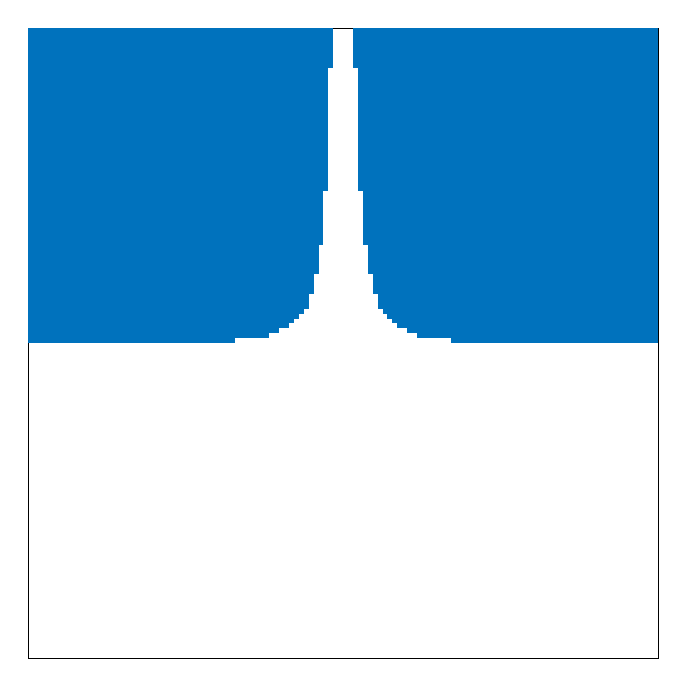
\begin{tikzpicture}
\footnotesize

\begin{axis}[%
width=8cm,
height=8cm,
at={(0in,0in)},
scale only axis,
unbounded coords=jump,
xmin=-8,
xmax=8,
xtick={\empty},
ymin=-8,
ymax=8,
ytick={\empty},
axis background/.style={fill=white}
]
\addplot [color=mycolor1, forget plot]
  table[row sep=crcr]{%
nan	nan\\
};

\addplot[area legend, draw=none, fill=mycolor1, forget plot]
table[row sep=crcr] {%
x	y\\
-8	0\\
-7.875	0\\
-7.875	0.125\\
-8	0.125\\
-8	0\\
}--cycle;

\addplot[area legend, draw=none, fill=mycolor1, forget plot]
table[row sep=crcr] {%
x	y\\
-8	0.125\\
-7.875	0.125\\
-7.875	0.25\\
-8	0.25\\
-8	0.125\\
}--cycle;

\addplot[area legend, draw=none, fill=mycolor1, forget plot]
table[row sep=crcr] {%
x	y\\
-7.875	0\\
-7.75	0\\
-7.75	0.125\\
-7.875	0.125\\
-7.875	0\\
}--cycle;

\addplot[area legend, draw=none, fill=mycolor1, forget plot]
table[row sep=crcr] {%
x	y\\
-7.875	0.125\\
-7.75	0.125\\
-7.75	0.25\\
-7.875	0.25\\
-7.875	0.125\\
}--cycle;

\addplot[area legend, draw=none, fill=mycolor1, forget plot]
table[row sep=crcr] {%
x	y\\
-8	0.25\\
-7.75	0.25\\
-7.75	0.5\\
-8	0.5\\
-8	0.25\\
}--cycle;

\addplot[area legend, draw=none, fill=mycolor1, forget plot]
table[row sep=crcr] {%
x	y\\
-7.75	0\\
-7.625	0\\
-7.625	0.125\\
-7.75	0.125\\
-7.75	0\\
}--cycle;

\addplot[area legend, draw=none, fill=mycolor1, forget plot]
table[row sep=crcr] {%
x	y\\
-7.75	0.125\\
-7.625	0.125\\
-7.625	0.25\\
-7.75	0.25\\
-7.75	0.125\\
}--cycle;

\addplot[area legend, draw=none, fill=mycolor1, forget plot]
table[row sep=crcr] {%
x	y\\
-7.625	0\\
-7.5	0\\
-7.5	0.125\\
-7.625	0.125\\
-7.625	0\\
}--cycle;

\addplot[area legend, draw=none, fill=mycolor1, forget plot]
table[row sep=crcr] {%
x	y\\
-7.625	0.125\\
-7.5	0.125\\
-7.5	0.25\\
-7.625	0.25\\
-7.625	0.125\\
}--cycle;

\addplot[area legend, draw=none, fill=mycolor1, forget plot]
table[row sep=crcr] {%
x	y\\
-7.75	0.25\\
-7.5	0.25\\
-7.5	0.5\\
-7.75	0.5\\
-7.75	0.25\\
}--cycle;

\addplot[area legend, draw=none, fill=mycolor1, forget plot]
table[row sep=crcr] {%
x	y\\
-8	0.5\\
-7.5	0.5\\
-7.5	1\\
-8	1\\
-8	0.5\\
}--cycle;

\addplot[area legend, draw=none, fill=mycolor1, forget plot]
table[row sep=crcr] {%
x	y\\
-7.5	0\\
-7.375	0\\
-7.375	0.125\\
-7.5	0.125\\
-7.5	0\\
}--cycle;

\addplot[area legend, draw=none, fill=mycolor1, forget plot]
table[row sep=crcr] {%
x	y\\
-7.5	0.125\\
-7.375	0.125\\
-7.375	0.25\\
-7.5	0.25\\
-7.5	0.125\\
}--cycle;

\addplot[area legend, draw=none, fill=mycolor1, forget plot]
table[row sep=crcr] {%
x	y\\
-7.375	0\\
-7.25	0\\
-7.25	0.125\\
-7.375	0.125\\
-7.375	0\\
}--cycle;

\addplot[area legend, draw=none, fill=mycolor1, forget plot]
table[row sep=crcr] {%
x	y\\
-7.375	0.125\\
-7.25	0.125\\
-7.25	0.25\\
-7.375	0.25\\
-7.375	0.125\\
}--cycle;

\addplot[area legend, draw=none, fill=mycolor1, forget plot]
table[row sep=crcr] {%
x	y\\
-7.5	0.25\\
-7.25	0.25\\
-7.25	0.5\\
-7.5	0.5\\
-7.5	0.25\\
}--cycle;

\addplot[area legend, draw=none, fill=mycolor1, forget plot]
table[row sep=crcr] {%
x	y\\
-7.25	0\\
-7.125	0\\
-7.125	0.125\\
-7.25	0.125\\
-7.25	0\\
}--cycle;

\addplot[area legend, draw=none, fill=mycolor1, forget plot]
table[row sep=crcr] {%
x	y\\
-7.25	0.125\\
-7.125	0.125\\
-7.125	0.25\\
-7.25	0.25\\
-7.25	0.125\\
}--cycle;

\addplot[area legend, draw=none, fill=mycolor1, forget plot]
table[row sep=crcr] {%
x	y\\
-7.125	0\\
-7	0\\
-7	0.125\\
-7.125	0.125\\
-7.125	0\\
}--cycle;

\addplot[area legend, draw=none, fill=mycolor1, forget plot]
table[row sep=crcr] {%
x	y\\
-7.125	0.125\\
-7	0.125\\
-7	0.25\\
-7.125	0.25\\
-7.125	0.125\\
}--cycle;

\addplot[area legend, draw=none, fill=mycolor1, forget plot]
table[row sep=crcr] {%
x	y\\
-7.25	0.25\\
-7	0.25\\
-7	0.5\\
-7.25	0.5\\
-7.25	0.25\\
}--cycle;

\addplot[area legend, draw=none, fill=mycolor1, forget plot]
table[row sep=crcr] {%
x	y\\
-7.5	0.5\\
-7	0.5\\
-7	1\\
-7.5	1\\
-7.5	0.5\\
}--cycle;

\addplot[area legend, draw=none, fill=mycolor1, forget plot]
table[row sep=crcr] {%
x	y\\
-8	1\\
-7	1\\
-7	2\\
-8	2\\
-8	1\\
}--cycle;

\addplot[area legend, draw=none, fill=mycolor1, forget plot]
table[row sep=crcr] {%
x	y\\
-7	0\\
-6.875	0\\
-6.875	0.125\\
-7	0.125\\
-7	0\\
}--cycle;

\addplot[area legend, draw=none, fill=mycolor1, forget plot]
table[row sep=crcr] {%
x	y\\
-7	0.125\\
-6.875	0.125\\
-6.875	0.25\\
-7	0.25\\
-7	0.125\\
}--cycle;

\addplot[area legend, draw=none, fill=mycolor1, forget plot]
table[row sep=crcr] {%
x	y\\
-6.875	0\\
-6.75	0\\
-6.75	0.125\\
-6.875	0.125\\
-6.875	0\\
}--cycle;

\addplot[area legend, draw=none, fill=mycolor1, forget plot]
table[row sep=crcr] {%
x	y\\
-6.875	0.125\\
-6.75	0.125\\
-6.75	0.25\\
-6.875	0.25\\
-6.875	0.125\\
}--cycle;

\addplot[area legend, draw=none, fill=mycolor1, forget plot]
table[row sep=crcr] {%
x	y\\
-7	0.25\\
-6.75	0.25\\
-6.75	0.5\\
-7	0.5\\
-7	0.25\\
}--cycle;

\addplot[area legend, draw=none, fill=mycolor1, forget plot]
table[row sep=crcr] {%
x	y\\
-6.75	0\\
-6.625	0\\
-6.625	0.125\\
-6.75	0.125\\
-6.75	0\\
}--cycle;

\addplot[area legend, draw=none, fill=mycolor1, forget plot]
table[row sep=crcr] {%
x	y\\
-6.75	0.125\\
-6.625	0.125\\
-6.625	0.25\\
-6.75	0.25\\
-6.75	0.125\\
}--cycle;

\addplot[area legend, draw=none, fill=mycolor1, forget plot]
table[row sep=crcr] {%
x	y\\
-6.625	0\\
-6.5	0\\
-6.5	0.125\\
-6.625	0.125\\
-6.625	0\\
}--cycle;

\addplot[area legend, draw=none, fill=mycolor1, forget plot]
table[row sep=crcr] {%
x	y\\
-6.625	0.125\\
-6.5	0.125\\
-6.5	0.25\\
-6.625	0.25\\
-6.625	0.125\\
}--cycle;

\addplot[area legend, draw=none, fill=mycolor1, forget plot]
table[row sep=crcr] {%
x	y\\
-6.75	0.25\\
-6.5	0.25\\
-6.5	0.5\\
-6.75	0.5\\
-6.75	0.25\\
}--cycle;

\addplot[area legend, draw=none, fill=mycolor1, forget plot]
table[row sep=crcr] {%
x	y\\
-7	0.5\\
-6.5	0.5\\
-6.5	1\\
-7	1\\
-7	0.5\\
}--cycle;

\addplot[area legend, draw=none, fill=mycolor1, forget plot]
table[row sep=crcr] {%
x	y\\
-6.5	0\\
-6.375	0\\
-6.375	0.125\\
-6.5	0.125\\
-6.5	0\\
}--cycle;

\addplot[area legend, draw=none, fill=mycolor1, forget plot]
table[row sep=crcr] {%
x	y\\
-6.5	0.125\\
-6.375	0.125\\
-6.375	0.25\\
-6.5	0.25\\
-6.5	0.125\\
}--cycle;

\addplot[area legend, draw=none, fill=mycolor1, forget plot]
table[row sep=crcr] {%
x	y\\
-6.375	0\\
-6.25	0\\
-6.25	0.125\\
-6.375	0.125\\
-6.375	0\\
}--cycle;

\addplot[area legend, draw=none, fill=mycolor1, forget plot]
table[row sep=crcr] {%
x	y\\
-6.375	0.125\\
-6.25	0.125\\
-6.25	0.25\\
-6.375	0.25\\
-6.375	0.125\\
}--cycle;

\addplot[area legend, draw=none, fill=mycolor1, forget plot]
table[row sep=crcr] {%
x	y\\
-6.5	0.25\\
-6.25	0.25\\
-6.25	0.5\\
-6.5	0.5\\
-6.5	0.25\\
}--cycle;

\addplot[area legend, draw=none, fill=mycolor1, forget plot]
table[row sep=crcr] {%
x	y\\
-6.25	0\\
-6.125	0\\
-6.125	0.125\\
-6.25	0.125\\
-6.25	0\\
}--cycle;

\addplot[area legend, draw=none, fill=mycolor1, forget plot]
table[row sep=crcr] {%
x	y\\
-6.25	0.125\\
-6.125	0.125\\
-6.125	0.25\\
-6.25	0.25\\
-6.25	0.125\\
}--cycle;

\addplot[area legend, draw=none, fill=mycolor1, forget plot]
table[row sep=crcr] {%
x	y\\
-6.125	0\\
-6	0\\
-6	0.125\\
-6.125	0.125\\
-6.125	0\\
}--cycle;

\addplot[area legend, draw=none, fill=mycolor1, forget plot]
table[row sep=crcr] {%
x	y\\
-6.125	0.125\\
-6	0.125\\
-6	0.25\\
-6.125	0.25\\
-6.125	0.125\\
}--cycle;

\addplot[area legend, draw=none, fill=mycolor1, forget plot]
table[row sep=crcr] {%
x	y\\
-6.25	0.25\\
-6	0.25\\
-6	0.5\\
-6.25	0.5\\
-6.25	0.25\\
}--cycle;

\addplot[area legend, draw=none, fill=mycolor1, forget plot]
table[row sep=crcr] {%
x	y\\
-6.5	0.5\\
-6	0.5\\
-6	1\\
-6.5	1\\
-6.5	0.5\\
}--cycle;

\addplot[area legend, draw=none, fill=mycolor1, forget plot]
table[row sep=crcr] {%
x	y\\
-7	1\\
-6	1\\
-6	2\\
-7	2\\
-7	1\\
}--cycle;

\addplot[area legend, draw=none, fill=mycolor1, forget plot]
table[row sep=crcr] {%
x	y\\
-8	2\\
-6	2\\
-6	4\\
-8	4\\
-8	2\\
}--cycle;

\addplot[area legend, draw=none, fill=mycolor1, forget plot]
table[row sep=crcr] {%
x	y\\
-6	0\\
-5.875	0\\
-5.875	0.125\\
-6	0.125\\
-6	0\\
}--cycle;

\addplot[area legend, draw=none, fill=mycolor1, forget plot]
table[row sep=crcr] {%
x	y\\
-6	0.125\\
-5.875	0.125\\
-5.875	0.25\\
-6	0.25\\
-6	0.125\\
}--cycle;

\addplot[area legend, draw=none, fill=mycolor1, forget plot]
table[row sep=crcr] {%
x	y\\
-5.875	0\\
-5.75	0\\
-5.75	0.125\\
-5.875	0.125\\
-5.875	0\\
}--cycle;

\addplot[area legend, draw=none, fill=mycolor1, forget plot]
table[row sep=crcr] {%
x	y\\
-5.875	0.125\\
-5.75	0.125\\
-5.75	0.25\\
-5.875	0.25\\
-5.875	0.125\\
}--cycle;

\addplot[area legend, draw=none, fill=mycolor1, forget plot]
table[row sep=crcr] {%
x	y\\
-6	0.25\\
-5.75	0.25\\
-5.75	0.5\\
-6	0.5\\
-6	0.25\\
}--cycle;

\addplot[area legend, draw=none, fill=mycolor1, forget plot]
table[row sep=crcr] {%
x	y\\
-5.75	0\\
-5.625	0\\
-5.625	0.125\\
-5.75	0.125\\
-5.75	0\\
}--cycle;

\addplot[area legend, draw=none, fill=mycolor1, forget plot]
table[row sep=crcr] {%
x	y\\
-5.75	0.125\\
-5.625	0.125\\
-5.625	0.25\\
-5.75	0.25\\
-5.75	0.125\\
}--cycle;

\addplot[area legend, draw=none, fill=mycolor1, forget plot]
table[row sep=crcr] {%
x	y\\
-5.625	0\\
-5.5	0\\
-5.5	0.125\\
-5.625	0.125\\
-5.625	0\\
}--cycle;

\addplot[area legend, draw=none, fill=mycolor1, forget plot]
table[row sep=crcr] {%
x	y\\
-5.625	0.125\\
-5.5	0.125\\
-5.5	0.25\\
-5.625	0.25\\
-5.625	0.125\\
}--cycle;

\addplot[area legend, draw=none, fill=mycolor1, forget plot]
table[row sep=crcr] {%
x	y\\
-5.75	0.25\\
-5.5	0.25\\
-5.5	0.5\\
-5.75	0.5\\
-5.75	0.25\\
}--cycle;

\addplot[area legend, draw=none, fill=mycolor1, forget plot]
table[row sep=crcr] {%
x	y\\
-6	0.5\\
-5.5	0.5\\
-5.5	1\\
-6	1\\
-6	0.5\\
}--cycle;

\addplot[area legend, draw=none, fill=mycolor1, forget plot]
table[row sep=crcr] {%
x	y\\
-5.5	0\\
-5.375	0\\
-5.375	0.125\\
-5.5	0.125\\
-5.5	0\\
}--cycle;

\addplot[area legend, draw=none, fill=mycolor1, forget plot]
table[row sep=crcr] {%
x	y\\
-5.5	0.125\\
-5.375	0.125\\
-5.375	0.25\\
-5.5	0.25\\
-5.5	0.125\\
}--cycle;

\addplot[area legend, draw=none, fill=mycolor1, forget plot]
table[row sep=crcr] {%
x	y\\
-5.375	0\\
-5.25	0\\
-5.25	0.125\\
-5.375	0.125\\
-5.375	0\\
}--cycle;

\addplot[area legend, draw=none, fill=mycolor1, forget plot]
table[row sep=crcr] {%
x	y\\
-5.375	0.125\\
-5.25	0.125\\
-5.25	0.25\\
-5.375	0.25\\
-5.375	0.125\\
}--cycle;

\addplot[area legend, draw=none, fill=mycolor1, forget plot]
table[row sep=crcr] {%
x	y\\
-5.5	0.25\\
-5.25	0.25\\
-5.25	0.5\\
-5.5	0.5\\
-5.5	0.25\\
}--cycle;

\addplot[area legend, draw=none, fill=mycolor1, forget plot]
table[row sep=crcr] {%
x	y\\
-5.25	0\\
-5.125	0\\
-5.125	0.125\\
-5.25	0.125\\
-5.25	0\\
}--cycle;

\addplot[area legend, draw=none, fill=mycolor1, forget plot]
table[row sep=crcr] {%
x	y\\
-5.25	0.125\\
-5.125	0.125\\
-5.125	0.25\\
-5.25	0.25\\
-5.25	0.125\\
}--cycle;

\addplot[area legend, draw=none, fill=mycolor1, forget plot]
table[row sep=crcr] {%
x	y\\
-5.125	0\\
-5	0\\
-5	0.125\\
-5.125	0.125\\
-5.125	0\\
}--cycle;

\addplot[area legend, draw=none, fill=mycolor1, forget plot]
table[row sep=crcr] {%
x	y\\
-5.125	0.125\\
-5	0.125\\
-5	0.25\\
-5.125	0.25\\
-5.125	0.125\\
}--cycle;

\addplot[area legend, draw=none, fill=mycolor1, forget plot]
table[row sep=crcr] {%
x	y\\
-5.25	0.25\\
-5	0.25\\
-5	0.5\\
-5.25	0.5\\
-5.25	0.25\\
}--cycle;

\addplot[area legend, draw=none, fill=mycolor1, forget plot]
table[row sep=crcr] {%
x	y\\
-5.5	0.5\\
-5	0.5\\
-5	1\\
-5.5	1\\
-5.5	0.5\\
}--cycle;

\addplot[area legend, draw=none, fill=mycolor1, forget plot]
table[row sep=crcr] {%
x	y\\
-6	1\\
-5	1\\
-5	2\\
-6	2\\
-6	1\\
}--cycle;

\addplot[area legend, draw=none, fill=mycolor1, forget plot]
table[row sep=crcr] {%
x	y\\
-5	0\\
-4.875	0\\
-4.875	0.125\\
-5	0.125\\
-5	0\\
}--cycle;

\addplot[area legend, draw=none, fill=mycolor1, forget plot]
table[row sep=crcr] {%
x	y\\
-5	0.125\\
-4.875	0.125\\
-4.875	0.25\\
-5	0.25\\
-5	0.125\\
}--cycle;

\addplot[area legend, draw=none, fill=mycolor1, forget plot]
table[row sep=crcr] {%
x	y\\
-4.875	0\\
-4.75	0\\
-4.75	0.125\\
-4.875	0.125\\
-4.875	0\\
}--cycle;

\addplot[area legend, draw=none, fill=mycolor1, forget plot]
table[row sep=crcr] {%
x	y\\
-4.875	0.125\\
-4.75	0.125\\
-4.75	0.25\\
-4.875	0.25\\
-4.875	0.125\\
}--cycle;

\addplot[area legend, draw=none, fill=mycolor1, forget plot]
table[row sep=crcr] {%
x	y\\
-5	0.25\\
-4.75	0.25\\
-4.75	0.5\\
-5	0.5\\
-5	0.25\\
}--cycle;

\addplot[area legend, draw=none, fill=mycolor1, forget plot]
table[row sep=crcr] {%
x	y\\
-4.75	0\\
-4.625	0\\
-4.625	0.125\\
-4.75	0.125\\
-4.75	0\\
}--cycle;

\addplot[area legend, draw=none, fill=mycolor1, forget plot]
table[row sep=crcr] {%
x	y\\
-4.75	0.125\\
-4.625	0.125\\
-4.625	0.25\\
-4.75	0.25\\
-4.75	0.125\\
}--cycle;

\addplot[area legend, draw=none, fill=mycolor1, forget plot]
table[row sep=crcr] {%
x	y\\
-4.625	0\\
-4.5	0\\
-4.5	0.125\\
-4.625	0.125\\
-4.625	0\\
}--cycle;

\addplot[area legend, draw=none, fill=mycolor1, forget plot]
table[row sep=crcr] {%
x	y\\
-4.625	0.125\\
-4.5	0.125\\
-4.5	0.25\\
-4.625	0.25\\
-4.625	0.125\\
}--cycle;

\addplot[area legend, draw=none, fill=mycolor1, forget plot]
table[row sep=crcr] {%
x	y\\
-4.75	0.25\\
-4.5	0.25\\
-4.5	0.5\\
-4.75	0.5\\
-4.75	0.25\\
}--cycle;

\addplot[area legend, draw=none, fill=mycolor1, forget plot]
table[row sep=crcr] {%
x	y\\
-5	0.5\\
-4.5	0.5\\
-4.5	1\\
-5	1\\
-5	0.5\\
}--cycle;

\addplot[area legend, draw=none, fill=mycolor1, forget plot]
table[row sep=crcr] {%
x	y\\
-4.5	0\\
-4.375	0\\
-4.375	0.125\\
-4.5	0.125\\
-4.5	0\\
}--cycle;

\addplot[area legend, draw=none, fill=mycolor1, forget plot]
table[row sep=crcr] {%
x	y\\
-4.5	0.125\\
-4.375	0.125\\
-4.375	0.25\\
-4.5	0.25\\
-4.5	0.125\\
}--cycle;

\addplot[area legend, draw=none, fill=mycolor1, forget plot]
table[row sep=crcr] {%
x	y\\
-4.375	0\\
-4.25	0\\
-4.25	0.125\\
-4.375	0.125\\
-4.375	0\\
}--cycle;

\addplot[area legend, draw=none, fill=mycolor1, forget plot]
table[row sep=crcr] {%
x	y\\
-4.375	0.125\\
-4.25	0.125\\
-4.25	0.25\\
-4.375	0.25\\
-4.375	0.125\\
}--cycle;

\addplot[area legend, draw=none, fill=mycolor1, forget plot]
table[row sep=crcr] {%
x	y\\
-4.5	0.25\\
-4.25	0.25\\
-4.25	0.5\\
-4.5	0.5\\
-4.5	0.25\\
}--cycle;

\addplot[area legend, draw=none, fill=mycolor1, forget plot]
table[row sep=crcr] {%
x	y\\
-4.25	0\\
-4.125	0\\
-4.125	0.125\\
-4.25	0.125\\
-4.25	0\\
}--cycle;

\addplot[area legend, draw=none, fill=mycolor1, forget plot]
table[row sep=crcr] {%
x	y\\
-4.25	0.125\\
-4.125	0.125\\
-4.125	0.25\\
-4.25	0.25\\
-4.25	0.125\\
}--cycle;

\addplot[area legend, draw=none, fill=mycolor1, forget plot]
table[row sep=crcr] {%
x	y\\
-4.125	0\\
-4	0\\
-4	0.125\\
-4.125	0.125\\
-4.125	0\\
}--cycle;

\addplot[area legend, draw=none, fill=mycolor1, forget plot]
table[row sep=crcr] {%
x	y\\
-4.125	0.125\\
-4	0.125\\
-4	0.25\\
-4.125	0.25\\
-4.125	0.125\\
}--cycle;

\addplot[area legend, draw=none, fill=mycolor1, forget plot]
table[row sep=crcr] {%
x	y\\
-4.25	0.25\\
-4	0.25\\
-4	0.5\\
-4.25	0.5\\
-4.25	0.25\\
}--cycle;

\addplot[area legend, draw=none, fill=mycolor1, forget plot]
table[row sep=crcr] {%
x	y\\
-4.5	0.5\\
-4	0.5\\
-4	1\\
-4.5	1\\
-4.5	0.5\\
}--cycle;

\addplot[area legend, draw=none, fill=mycolor1, forget plot]
table[row sep=crcr] {%
x	y\\
-5	1\\
-4	1\\
-4	2\\
-5	2\\
-5	1\\
}--cycle;

\addplot[area legend, draw=none, fill=mycolor1, forget plot]
table[row sep=crcr] {%
x	y\\
-6	2\\
-4	2\\
-4	4\\
-6	4\\
-6	2\\
}--cycle;

\addplot[area legend, draw=none, fill=mycolor1, forget plot]
table[row sep=crcr] {%
x	y\\
-8	4\\
-4	4\\
-4	8\\
-8	8\\
-8	4\\
}--cycle;

\addplot[area legend, draw=none, fill=mycolor1, forget plot]
table[row sep=crcr] {%
x	y\\
-4	0\\
-3.875	0\\
-3.875	0.125\\
-4	0.125\\
-4	0\\
}--cycle;

\addplot[area legend, draw=none, fill=mycolor1, forget plot]
table[row sep=crcr] {%
x	y\\
-4	0.125\\
-3.875	0.125\\
-3.875	0.25\\
-4	0.25\\
-4	0.125\\
}--cycle;

\addplot[area legend, draw=none, fill=mycolor1, forget plot]
table[row sep=crcr] {%
x	y\\
-3.875	0\\
-3.75	0\\
-3.75	0.125\\
-3.875	0.125\\
-3.875	0\\
}--cycle;

\addplot[area legend, draw=none, fill=mycolor1, forget plot]
table[row sep=crcr] {%
x	y\\
-3.875	0.125\\
-3.75	0.125\\
-3.75	0.25\\
-3.875	0.25\\
-3.875	0.125\\
}--cycle;

\addplot[area legend, draw=none, fill=mycolor1, forget plot]
table[row sep=crcr] {%
x	y\\
-4	0.25\\
-3.75	0.25\\
-3.75	0.5\\
-4	0.5\\
-4	0.25\\
}--cycle;

\addplot[area legend, draw=none, fill=mycolor1, forget plot]
table[row sep=crcr] {%
x	y\\
-3.75	0\\
-3.625	0\\
-3.625	0.125\\
-3.75	0.125\\
-3.75	0\\
}--cycle;

\addplot[area legend, draw=none, fill=mycolor1, forget plot]
table[row sep=crcr] {%
x	y\\
-3.75	0.125\\
-3.625	0.125\\
-3.625	0.25\\
-3.75	0.25\\
-3.75	0.125\\
}--cycle;

\addplot[area legend, draw=none, fill=mycolor1, forget plot]
table[row sep=crcr] {%
x	y\\
-3.625	0\\
-3.5	0\\
-3.5	0.125\\
-3.625	0.125\\
-3.625	0\\
}--cycle;

\addplot[area legend, draw=none, fill=mycolor1, forget plot]
table[row sep=crcr] {%
x	y\\
-3.625	0.125\\
-3.5	0.125\\
-3.5	0.25\\
-3.625	0.25\\
-3.625	0.125\\
}--cycle;

\addplot[area legend, draw=none, fill=mycolor1, forget plot]
table[row sep=crcr] {%
x	y\\
-3.75	0.25\\
-3.5	0.25\\
-3.5	0.5\\
-3.75	0.5\\
-3.75	0.25\\
}--cycle;

\addplot[area legend, draw=none, fill=mycolor1, forget plot]
table[row sep=crcr] {%
x	y\\
-4	0.5\\
-3.5	0.5\\
-3.5	1\\
-4	1\\
-4	0.5\\
}--cycle;

\addplot[area legend, draw=none, fill=mycolor1, forget plot]
table[row sep=crcr] {%
x	y\\
-3.5	0\\
-3.375	0\\
-3.375	0.125\\
-3.5	0.125\\
-3.5	0\\
}--cycle;

\addplot[area legend, draw=none, fill=mycolor1, forget plot]
table[row sep=crcr] {%
x	y\\
-3.5	0.125\\
-3.375	0.125\\
-3.375	0.25\\
-3.5	0.25\\
-3.5	0.125\\
}--cycle;

\addplot[area legend, draw=none, fill=mycolor1, forget plot]
table[row sep=crcr] {%
x	y\\
-3.375	0\\
-3.25	0\\
-3.25	0.125\\
-3.375	0.125\\
-3.375	0\\
}--cycle;

\addplot[area legend, draw=none, fill=mycolor1, forget plot]
table[row sep=crcr] {%
x	y\\
-3.375	0.125\\
-3.25	0.125\\
-3.25	0.25\\
-3.375	0.25\\
-3.375	0.125\\
}--cycle;

\addplot[area legend, draw=none, fill=mycolor1, forget plot]
table[row sep=crcr] {%
x	y\\
-3.5	0.25\\
-3.25	0.25\\
-3.25	0.5\\
-3.5	0.5\\
-3.5	0.25\\
}--cycle;

\addplot[area legend, draw=none, fill=mycolor1, forget plot]
table[row sep=crcr] {%
x	y\\
-3.25	0\\
-3.125	0\\
-3.125	0.125\\
-3.25	0.125\\
-3.25	0\\
}--cycle;

\addplot[area legend, draw=none, fill=mycolor1, forget plot]
table[row sep=crcr] {%
x	y\\
-3.25	0.125\\
-3.125	0.125\\
-3.125	0.25\\
-3.25	0.25\\
-3.25	0.125\\
}--cycle;

\addplot[area legend, draw=none, fill=mycolor1, forget plot]
table[row sep=crcr] {%
x	y\\
-3.125	0\\
-3	0\\
-3	0.125\\
-3.125	0.125\\
-3.125	0\\
}--cycle;

\addplot[area legend, draw=none, fill=mycolor1, forget plot]
table[row sep=crcr] {%
x	y\\
-3.125	0.125\\
-3	0.125\\
-3	0.25\\
-3.125	0.25\\
-3.125	0.125\\
}--cycle;

\addplot[area legend, draw=none, fill=mycolor1, forget plot]
table[row sep=crcr] {%
x	y\\
-3.25	0.25\\
-3	0.25\\
-3	0.5\\
-3.25	0.5\\
-3.25	0.25\\
}--cycle;

\addplot[area legend, draw=none, fill=mycolor1, forget plot]
table[row sep=crcr] {%
x	y\\
-3.5	0.5\\
-3	0.5\\
-3	1\\
-3.5	1\\
-3.5	0.5\\
}--cycle;

\addplot[area legend, draw=none, fill=mycolor1, forget plot]
table[row sep=crcr] {%
x	y\\
-4	1\\
-3	1\\
-3	2\\
-4	2\\
-4	1\\
}--cycle;

\addplot[area legend, draw=none, fill=mycolor1, forget plot]
table[row sep=crcr] {%
x	y\\
-3	0\\
-2.875	0\\
-2.875	0.125\\
-3	0.125\\
-3	0\\
}--cycle;

\addplot[area legend, draw=none, fill=mycolor1, forget plot]
table[row sep=crcr] {%
x	y\\
-3	0.125\\
-2.875	0.125\\
-2.875	0.25\\
-3	0.25\\
-3	0.125\\
}--cycle;

\addplot[area legend, draw=none, fill=mycolor1, forget plot]
table[row sep=crcr] {%
x	y\\
-2.875	0\\
-2.75	0\\
-2.75	0.125\\
-2.875	0.125\\
-2.875	0\\
}--cycle;

\addplot[area legend, draw=none, fill=mycolor1, forget plot]
table[row sep=crcr] {%
x	y\\
-2.875	0.125\\
-2.75	0.125\\
-2.75	0.25\\
-2.875	0.25\\
-2.875	0.125\\
}--cycle;

\addplot[area legend, draw=none, fill=mycolor1, forget plot]
table[row sep=crcr] {%
x	y\\
-3	0.25\\
-2.75	0.25\\
-2.75	0.5\\
-3	0.5\\
-3	0.25\\
}--cycle;

\addplot[area legend, draw=none, fill=mycolor1, forget plot]
table[row sep=crcr] {%
x	y\\
-2.75	0.125\\
-2.625	0.125\\
-2.625	0.25\\
-2.75	0.25\\
-2.75	0.125\\
}--cycle;

\addplot[area legend, draw=none, fill=mycolor1, forget plot]
table[row sep=crcr] {%
x	y\\
-2.625	0.125\\
-2.5	0.125\\
-2.5	0.25\\
-2.625	0.25\\
-2.625	0.125\\
}--cycle;

\addplot[area legend, draw=none, fill=mycolor1, forget plot]
table[row sep=crcr] {%
x	y\\
-2.75	0.25\\
-2.5	0.25\\
-2.5	0.5\\
-2.75	0.5\\
-2.75	0.25\\
}--cycle;

\addplot[area legend, draw=none, fill=mycolor1, forget plot]
table[row sep=crcr] {%
x	y\\
-3	0.5\\
-2.5	0.5\\
-2.5	1\\
-3	1\\
-3	0.5\\
}--cycle;

\addplot[area legend, draw=none, fill=mycolor1, forget plot]
table[row sep=crcr] {%
x	y\\
-2.5	0.125\\
-2.375	0.125\\
-2.375	0.25\\
-2.5	0.25\\
-2.5	0.125\\
}--cycle;

\addplot[area legend, draw=none, fill=mycolor1, forget plot]
table[row sep=crcr] {%
x	y\\
-2.375	0.125\\
-2.25	0.125\\
-2.25	0.25\\
-2.375	0.25\\
-2.375	0.125\\
}--cycle;

\addplot[area legend, draw=none, fill=mycolor1, forget plot]
table[row sep=crcr] {%
x	y\\
-2.5	0.25\\
-2.25	0.25\\
-2.25	0.5\\
-2.5	0.5\\
-2.5	0.25\\
}--cycle;

\addplot[area legend, draw=none, fill=mycolor1, forget plot]
table[row sep=crcr] {%
x	y\\
-2.25	0.125\\
-2.125	0.125\\
-2.125	0.25\\
-2.25	0.25\\
-2.25	0.125\\
}--cycle;

\addplot[area legend, draw=none, fill=mycolor1, forget plot]
table[row sep=crcr] {%
x	y\\
-2.125	0.125\\
-2	0.125\\
-2	0.25\\
-2.125	0.25\\
-2.125	0.125\\
}--cycle;

\addplot[area legend, draw=none, fill=mycolor1, forget plot]
table[row sep=crcr] {%
x	y\\
-2.25	0.25\\
-2	0.25\\
-2	0.5\\
-2.25	0.5\\
-2.25	0.25\\
}--cycle;

\addplot[area legend, draw=none, fill=mycolor1, forget plot]
table[row sep=crcr] {%
x	y\\
-2.5	0.5\\
-2	0.5\\
-2	1\\
-2.5	1\\
-2.5	0.5\\
}--cycle;

\addplot[area legend, draw=none, fill=mycolor1, forget plot]
table[row sep=crcr] {%
x	y\\
-3	1\\
-2	1\\
-2	2\\
-3	2\\
-3	1\\
}--cycle;

\addplot[area legend, draw=none, fill=mycolor1, forget plot]
table[row sep=crcr] {%
x	y\\
-4	2\\
-2	2\\
-2	4\\
-4	4\\
-4	2\\
}--cycle;

\addplot[area legend, draw=none, fill=mycolor1, forget plot]
table[row sep=crcr] {%
x	y\\
-2	0.125\\
-1.875	0.125\\
-1.875	0.25\\
-2	0.25\\
-2	0.125\\
}--cycle;

\addplot[area legend, draw=none, fill=mycolor1, forget plot]
table[row sep=crcr] {%
x	y\\
-2	0.25\\
-1.875	0.25\\
-1.875	0.375\\
-2	0.375\\
-2	0.25\\
}--cycle;

\addplot[area legend, draw=none, fill=mycolor1, forget plot]
table[row sep=crcr] {%
x	y\\
-2	0.375\\
-1.875	0.375\\
-1.875	0.5\\
-2	0.5\\
-2	0.375\\
}--cycle;

\addplot[area legend, draw=none, fill=mycolor1, forget plot]
table[row sep=crcr] {%
x	y\\
-1.875	0.25\\
-1.75	0.25\\
-1.75	0.375\\
-1.875	0.375\\
-1.875	0.25\\
}--cycle;

\addplot[area legend, draw=none, fill=mycolor1, forget plot]
table[row sep=crcr] {%
x	y\\
-1.875	0.375\\
-1.75	0.375\\
-1.75	0.5\\
-1.875	0.5\\
-1.875	0.375\\
}--cycle;

\addplot[area legend, draw=none, fill=mycolor1, forget plot]
table[row sep=crcr] {%
x	y\\
-1.75	0.25\\
-1.625	0.25\\
-1.625	0.375\\
-1.75	0.375\\
-1.75	0.25\\
}--cycle;

\addplot[area legend, draw=none, fill=mycolor1, forget plot]
table[row sep=crcr] {%
x	y\\
-1.75	0.375\\
-1.625	0.375\\
-1.625	0.5\\
-1.75	0.5\\
-1.75	0.375\\
}--cycle;

\addplot[area legend, draw=none, fill=mycolor1, forget plot]
table[row sep=crcr] {%
x	y\\
-1.625	0.375\\
-1.5	0.375\\
-1.5	0.5\\
-1.625	0.5\\
-1.625	0.375\\
}--cycle;

\addplot[area legend, draw=none, fill=mycolor1, forget plot]
table[row sep=crcr] {%
x	y\\
-2	0.5\\
-1.5	0.5\\
-1.5	1\\
-2	1\\
-2	0.5\\
}--cycle;

\addplot[area legend, draw=none, fill=mycolor1, forget plot]
table[row sep=crcr] {%
x	y\\
-1.5	0.375\\
-1.375	0.375\\
-1.375	0.5\\
-1.5	0.5\\
-1.5	0.375\\
}--cycle;

\addplot[area legend, draw=none, fill=mycolor1, forget plot]
table[row sep=crcr] {%
x	y\\
-1.5	0.5\\
-1.375	0.5\\
-1.375	0.625\\
-1.5	0.625\\
-1.5	0.5\\
}--cycle;

\addplot[area legend, draw=none, fill=mycolor1, forget plot]
table[row sep=crcr] {%
x	y\\
-1.5	0.625\\
-1.375	0.625\\
-1.375	0.75\\
-1.5	0.75\\
-1.5	0.625\\
}--cycle;

\addplot[area legend, draw=none, fill=mycolor1, forget plot]
table[row sep=crcr] {%
x	y\\
-1.375	0.5\\
-1.25	0.5\\
-1.25	0.625\\
-1.375	0.625\\
-1.375	0.5\\
}--cycle;

\addplot[area legend, draw=none, fill=mycolor1, forget plot]
table[row sep=crcr] {%
x	y\\
-1.375	0.625\\
-1.25	0.625\\
-1.25	0.75\\
-1.375	0.75\\
-1.375	0.625\\
}--cycle;

\addplot[area legend, draw=none, fill=mycolor1, forget plot]
table[row sep=crcr] {%
x	y\\
-1.5	0.75\\
-1.25	0.75\\
-1.25	1\\
-1.5	1\\
-1.5	0.75\\
}--cycle;

\addplot[area legend, draw=none, fill=mycolor1, forget plot]
table[row sep=crcr] {%
x	y\\
-1.25	0.625\\
-1.125	0.625\\
-1.125	0.75\\
-1.25	0.75\\
-1.25	0.625\\
}--cycle;

\addplot[area legend, draw=none, fill=mycolor1, forget plot]
table[row sep=crcr] {%
x	y\\
-1.25	0.75\\
-1.125	0.75\\
-1.125	0.875\\
-1.25	0.875\\
-1.25	0.75\\
}--cycle;

\addplot[area legend, draw=none, fill=mycolor1, forget plot]
table[row sep=crcr] {%
x	y\\
-1.25	0.875\\
-1.125	0.875\\
-1.125	1\\
-1.25	1\\
-1.25	0.875\\
}--cycle;

\addplot[area legend, draw=none, fill=mycolor1, forget plot]
table[row sep=crcr] {%
x	y\\
-1.125	0.75\\
-1	0.75\\
-1	0.875\\
-1.125	0.875\\
-1.125	0.75\\
}--cycle;

\addplot[area legend, draw=none, fill=mycolor1, forget plot]
table[row sep=crcr] {%
x	y\\
-1.125	0.875\\
-1	0.875\\
-1	1\\
-1.125	1\\
-1.125	0.875\\
}--cycle;

\addplot[area legend, draw=none, fill=mycolor1, forget plot]
table[row sep=crcr] {%
x	y\\
-2	1\\
-1	1\\
-1	2\\
-2	2\\
-2	1\\
}--cycle;

\addplot[area legend, draw=none, fill=mycolor1, forget plot]
table[row sep=crcr] {%
x	y\\
-1	0.875\\
-0.875	0.875\\
-0.875	1\\
-1	1\\
-1	0.875\\
}--cycle;

\addplot[area legend, draw=none, fill=mycolor1, forget plot]
table[row sep=crcr] {%
x	y\\
-1	1\\
-0.875	1\\
-0.875	1.125\\
-1	1.125\\
-1	1\\
}--cycle;

\addplot[area legend, draw=none, fill=mycolor1, forget plot]
table[row sep=crcr] {%
x	y\\
-1	1.125\\
-0.875	1.125\\
-0.875	1.25\\
-1	1.25\\
-1	1.125\\
}--cycle;

\addplot[area legend, draw=none, fill=mycolor1, forget plot]
table[row sep=crcr] {%
x	y\\
-1	1.25\\
-0.875	1.25\\
-0.875	1.375\\
-1	1.375\\
-1	1.25\\
}--cycle;

\addplot[area legend, draw=none, fill=mycolor1, forget plot]
table[row sep=crcr] {%
x	y\\
-1	1.375\\
-0.875	1.375\\
-0.875	1.5\\
-1	1.5\\
-1	1.375\\
}--cycle;

\addplot[area legend, draw=none, fill=mycolor1, forget plot]
table[row sep=crcr] {%
x	y\\
-0.875	1.25\\
-0.75	1.25\\
-0.75	1.375\\
-0.875	1.375\\
-0.875	1.25\\
}--cycle;

\addplot[area legend, draw=none, fill=mycolor1, forget plot]
table[row sep=crcr] {%
x	y\\
-0.875	1.375\\
-0.75	1.375\\
-0.75	1.5\\
-0.875	1.5\\
-0.875	1.375\\
}--cycle;

\addplot[area legend, draw=none, fill=mycolor1, forget plot]
table[row sep=crcr] {%
x	y\\
-1	1.5\\
-0.875	1.5\\
-0.875	1.625\\
-1	1.625\\
-1	1.5\\
}--cycle;

\addplot[area legend, draw=none, fill=mycolor1, forget plot]
table[row sep=crcr] {%
x	y\\
-1	1.625\\
-0.875	1.625\\
-0.875	1.75\\
-1	1.75\\
-1	1.625\\
}--cycle;

\addplot[area legend, draw=none, fill=mycolor1, forget plot]
table[row sep=crcr] {%
x	y\\
-0.875	1.5\\
-0.75	1.5\\
-0.75	1.625\\
-0.875	1.625\\
-0.875	1.5\\
}--cycle;

\addplot[area legend, draw=none, fill=mycolor1, forget plot]
table[row sep=crcr] {%
x	y\\
-0.875	1.625\\
-0.75	1.625\\
-0.75	1.75\\
-0.875	1.75\\
-0.875	1.625\\
}--cycle;

\addplot[area legend, draw=none, fill=mycolor1, forget plot]
table[row sep=crcr] {%
x	y\\
-1	1.75\\
-0.875	1.75\\
-0.875	1.875\\
-1	1.875\\
-1	1.75\\
}--cycle;

\addplot[area legend, draw=none, fill=mycolor1, forget plot]
table[row sep=crcr] {%
x	y\\
-1	1.875\\
-0.875	1.875\\
-0.875	2\\
-1	2\\
-1	1.875\\
}--cycle;

\addplot[area legend, draw=none, fill=mycolor1, forget plot]
table[row sep=crcr] {%
x	y\\
-0.875	1.75\\
-0.75	1.75\\
-0.75	1.875\\
-0.875	1.875\\
-0.875	1.75\\
}--cycle;

\addplot[area legend, draw=none, fill=mycolor1, forget plot]
table[row sep=crcr] {%
x	y\\
-0.875	1.875\\
-0.75	1.875\\
-0.75	2\\
-0.875	2\\
-0.875	1.875\\
}--cycle;

\addplot[area legend, draw=none, fill=mycolor1, forget plot]
table[row sep=crcr] {%
x	y\\
-0.75	1.75\\
-0.625	1.75\\
-0.625	1.875\\
-0.75	1.875\\
-0.75	1.75\\
}--cycle;

\addplot[area legend, draw=none, fill=mycolor1, forget plot]
table[row sep=crcr] {%
x	y\\
-0.75	1.875\\
-0.625	1.875\\
-0.625	2\\
-0.75	2\\
-0.75	1.875\\
}--cycle;

\addplot[area legend, draw=none, fill=mycolor1, forget plot]
table[row sep=crcr] {%
x	y\\
-2	2\\
-1	2\\
-1	3\\
-2	3\\
-2	2\\
}--cycle;

\addplot[area legend, draw=none, fill=mycolor1, forget plot]
table[row sep=crcr] {%
x	y\\
-2	3\\
-1	3\\
-1	4\\
-2	4\\
-2	3\\
}--cycle;

\addplot[area legend, draw=none, fill=mycolor1, forget plot]
table[row sep=crcr] {%
x	y\\
-1	2\\
-0.75	2\\
-0.75	2.25\\
-1	2.25\\
-1	2\\
}--cycle;

\addplot[area legend, draw=none, fill=mycolor1, forget plot]
table[row sep=crcr] {%
x	y\\
-1	2.25\\
-0.75	2.25\\
-0.75	2.5\\
-1	2.5\\
-1	2.25\\
}--cycle;

\addplot[area legend, draw=none, fill=mycolor1, forget plot]
table[row sep=crcr] {%
x	y\\
-0.75	2\\
-0.625	2\\
-0.625	2.125\\
-0.75	2.125\\
-0.75	2\\
}--cycle;

\addplot[area legend, draw=none, fill=mycolor1, forget plot]
table[row sep=crcr] {%
x	y\\
-0.75	2.125\\
-0.625	2.125\\
-0.625	2.25\\
-0.75	2.25\\
-0.75	2.125\\
}--cycle;

\addplot[area legend, draw=none, fill=mycolor1, forget plot]
table[row sep=crcr] {%
x	y\\
-0.75	2.25\\
-0.625	2.25\\
-0.625	2.375\\
-0.75	2.375\\
-0.75	2.25\\
}--cycle;

\addplot[area legend, draw=none, fill=mycolor1, forget plot]
table[row sep=crcr] {%
x	y\\
-0.75	2.375\\
-0.625	2.375\\
-0.625	2.5\\
-0.75	2.5\\
-0.75	2.375\\
}--cycle;

\addplot[area legend, draw=none, fill=mycolor1, forget plot]
table[row sep=crcr] {%
x	y\\
-1	2.5\\
-0.75	2.5\\
-0.75	2.75\\
-1	2.75\\
-1	2.5\\
}--cycle;

\addplot[area legend, draw=none, fill=mycolor1, forget plot]
table[row sep=crcr] {%
x	y\\
-1	2.75\\
-0.75	2.75\\
-0.75	3\\
-1	3\\
-1	2.75\\
}--cycle;

\addplot[area legend, draw=none, fill=mycolor1, forget plot]
table[row sep=crcr] {%
x	y\\
-0.75	2.5\\
-0.625	2.5\\
-0.625	2.625\\
-0.75	2.625\\
-0.75	2.5\\
}--cycle;

\addplot[area legend, draw=none, fill=mycolor1, forget plot]
table[row sep=crcr] {%
x	y\\
-0.75	2.625\\
-0.625	2.625\\
-0.625	2.75\\
-0.75	2.75\\
-0.75	2.625\\
}--cycle;

\addplot[area legend, draw=none, fill=mycolor1, forget plot]
table[row sep=crcr] {%
x	y\\
-0.625	2.5\\
-0.5	2.5\\
-0.5	2.625\\
-0.625	2.625\\
-0.625	2.5\\
}--cycle;

\addplot[area legend, draw=none, fill=mycolor1, forget plot]
table[row sep=crcr] {%
x	y\\
-0.625	2.625\\
-0.5	2.625\\
-0.5	2.75\\
-0.625	2.75\\
-0.625	2.625\\
}--cycle;

\addplot[area legend, draw=none, fill=mycolor1, forget plot]
table[row sep=crcr] {%
x	y\\
-0.75	2.75\\
-0.625	2.75\\
-0.625	2.875\\
-0.75	2.875\\
-0.75	2.75\\
}--cycle;

\addplot[area legend, draw=none, fill=mycolor1, forget plot]
table[row sep=crcr] {%
x	y\\
-0.75	2.875\\
-0.625	2.875\\
-0.625	3\\
-0.75	3\\
-0.75	2.875\\
}--cycle;

\addplot[area legend, draw=none, fill=mycolor1, forget plot]
table[row sep=crcr] {%
x	y\\
-0.625	2.75\\
-0.5	2.75\\
-0.5	2.875\\
-0.625	2.875\\
-0.625	2.75\\
}--cycle;

\addplot[area legend, draw=none, fill=mycolor1, forget plot]
table[row sep=crcr] {%
x	y\\
-0.625	2.875\\
-0.5	2.875\\
-0.5	3\\
-0.625	3\\
-0.625	2.875\\
}--cycle;

\addplot[area legend, draw=none, fill=mycolor1, forget plot]
table[row sep=crcr] {%
x	y\\
-1	3\\
-0.75	3\\
-0.75	3.25\\
-1	3.25\\
-1	3\\
}--cycle;

\addplot[area legend, draw=none, fill=mycolor1, forget plot]
table[row sep=crcr] {%
x	y\\
-1	3.25\\
-0.75	3.25\\
-0.75	3.5\\
-1	3.5\\
-1	3.25\\
}--cycle;

\addplot[area legend, draw=none, fill=mycolor1, forget plot]
table[row sep=crcr] {%
x	y\\
-0.75	3\\
-0.625	3\\
-0.625	3.125\\
-0.75	3.125\\
-0.75	3\\
}--cycle;

\addplot[area legend, draw=none, fill=mycolor1, forget plot]
table[row sep=crcr] {%
x	y\\
-0.75	3.125\\
-0.625	3.125\\
-0.625	3.25\\
-0.75	3.25\\
-0.75	3.125\\
}--cycle;

\addplot[area legend, draw=none, fill=mycolor1, forget plot]
table[row sep=crcr] {%
x	y\\
-0.625	3\\
-0.5	3\\
-0.5	3.125\\
-0.625	3.125\\
-0.625	3\\
}--cycle;

\addplot[area legend, draw=none, fill=mycolor1, forget plot]
table[row sep=crcr] {%
x	y\\
-0.625	3.125\\
-0.5	3.125\\
-0.5	3.25\\
-0.625	3.25\\
-0.625	3.125\\
}--cycle;

\addplot[area legend, draw=none, fill=mycolor1, forget plot]
table[row sep=crcr] {%
x	y\\
-0.75	3.25\\
-0.625	3.25\\
-0.625	3.375\\
-0.75	3.375\\
-0.75	3.25\\
}--cycle;

\addplot[area legend, draw=none, fill=mycolor1, forget plot]
table[row sep=crcr] {%
x	y\\
-0.75	3.375\\
-0.625	3.375\\
-0.625	3.5\\
-0.75	3.5\\
-0.75	3.375\\
}--cycle;

\addplot[area legend, draw=none, fill=mycolor1, forget plot]
table[row sep=crcr] {%
x	y\\
-0.625	3.25\\
-0.5	3.25\\
-0.5	3.375\\
-0.625	3.375\\
-0.625	3.25\\
}--cycle;

\addplot[area legend, draw=none, fill=mycolor1, forget plot]
table[row sep=crcr] {%
x	y\\
-0.625	3.375\\
-0.5	3.375\\
-0.5	3.5\\
-0.625	3.5\\
-0.625	3.375\\
}--cycle;

\addplot[area legend, draw=none, fill=mycolor1, forget plot]
table[row sep=crcr] {%
x	y\\
-1	3.5\\
-0.75	3.5\\
-0.75	3.75\\
-1	3.75\\
-1	3.5\\
}--cycle;

\addplot[area legend, draw=none, fill=mycolor1, forget plot]
table[row sep=crcr] {%
x	y\\
-1	3.75\\
-0.75	3.75\\
-0.75	4\\
-1	4\\
-1	3.75\\
}--cycle;

\addplot[area legend, draw=none, fill=mycolor1, forget plot]
table[row sep=crcr] {%
x	y\\
-0.75	3.5\\
-0.625	3.5\\
-0.625	3.625\\
-0.75	3.625\\
-0.75	3.5\\
}--cycle;

\addplot[area legend, draw=none, fill=mycolor1, forget plot]
table[row sep=crcr] {%
x	y\\
-0.75	3.625\\
-0.625	3.625\\
-0.625	3.75\\
-0.75	3.75\\
-0.75	3.625\\
}--cycle;

\addplot[area legend, draw=none, fill=mycolor1, forget plot]
table[row sep=crcr] {%
x	y\\
-0.625	3.5\\
-0.5	3.5\\
-0.5	3.625\\
-0.625	3.625\\
-0.625	3.5\\
}--cycle;

\addplot[area legend, draw=none, fill=mycolor1, forget plot]
table[row sep=crcr] {%
x	y\\
-0.625	3.625\\
-0.5	3.625\\
-0.5	3.75\\
-0.625	3.75\\
-0.625	3.625\\
}--cycle;

\addplot[area legend, draw=none, fill=mycolor1, forget plot]
table[row sep=crcr] {%
x	y\\
-0.75	3.75\\
-0.625	3.75\\
-0.625	3.875\\
-0.75	3.875\\
-0.75	3.75\\
}--cycle;

\addplot[area legend, draw=none, fill=mycolor1, forget plot]
table[row sep=crcr] {%
x	y\\
-0.75	3.875\\
-0.625	3.875\\
-0.625	4\\
-0.75	4\\
-0.75	3.875\\
}--cycle;

\addplot[area legend, draw=none, fill=mycolor1, forget plot]
table[row sep=crcr] {%
x	y\\
-0.625	3.75\\
-0.5	3.75\\
-0.5	3.875\\
-0.625	3.875\\
-0.625	3.75\\
}--cycle;

\addplot[area legend, draw=none, fill=mycolor1, forget plot]
table[row sep=crcr] {%
x	y\\
-0.625	3.875\\
-0.5	3.875\\
-0.5	4\\
-0.625	4\\
-0.625	3.875\\
}--cycle;

\addplot[area legend, draw=none, fill=mycolor1, forget plot]
table[row sep=crcr] {%
x	y\\
-0.5	3.875\\
-0.375	3.875\\
-0.375	4\\
-0.5	4\\
-0.5	3.875\\
}--cycle;

\addplot[area legend, draw=none, fill=mycolor1, forget plot]
table[row sep=crcr] {%
x	y\\
-4	4\\
-2	4\\
-2	6\\
-4	6\\
-4	4\\
}--cycle;

\addplot[area legend, draw=none, fill=mycolor1, forget plot]
table[row sep=crcr] {%
x	y\\
-4	6\\
-2	6\\
-2	8\\
-4	8\\
-4	6\\
}--cycle;

\addplot[area legend, draw=none, fill=mycolor1, forget plot]
table[row sep=crcr] {%
x	y\\
-2	4\\
-1	4\\
-1	5\\
-2	5\\
-2	4\\
}--cycle;

\addplot[area legend, draw=none, fill=mycolor1, forget plot]
table[row sep=crcr] {%
x	y\\
-2	5\\
-1	5\\
-1	6\\
-2	6\\
-2	5\\
}--cycle;

\addplot[area legend, draw=none, fill=mycolor1, forget plot]
table[row sep=crcr] {%
x	y\\
-1	4\\
-0.5	4\\
-0.5	4.5\\
-1	4.5\\
-1	4\\
}--cycle;

\addplot[area legend, draw=none, fill=mycolor1, forget plot]
table[row sep=crcr] {%
x	y\\
-1	4.5\\
-0.5	4.5\\
-0.5	5\\
-1	5\\
-1	4.5\\
}--cycle;

\addplot[area legend, draw=none, fill=mycolor1, forget plot]
table[row sep=crcr] {%
x	y\\
-0.5	4\\
-0.375	4\\
-0.375	4.125\\
-0.5	4.125\\
-0.5	4\\
}--cycle;

\addplot[area legend, draw=none, fill=mycolor1, forget plot]
table[row sep=crcr] {%
x	y\\
-0.5	4.125\\
-0.375	4.125\\
-0.375	4.25\\
-0.5	4.25\\
-0.5	4.125\\
}--cycle;

\addplot[area legend, draw=none, fill=mycolor1, forget plot]
table[row sep=crcr] {%
x	y\\
-0.5	4.25\\
-0.375	4.25\\
-0.375	4.375\\
-0.5	4.375\\
-0.5	4.25\\
}--cycle;

\addplot[area legend, draw=none, fill=mycolor1, forget plot]
table[row sep=crcr] {%
x	y\\
-0.5	4.375\\
-0.375	4.375\\
-0.375	4.5\\
-0.5	4.5\\
-0.5	4.375\\
}--cycle;

\addplot[area legend, draw=none, fill=mycolor1, forget plot]
table[row sep=crcr] {%
x	y\\
-0.5	4.5\\
-0.375	4.5\\
-0.375	4.625\\
-0.5	4.625\\
-0.5	4.5\\
}--cycle;

\addplot[area legend, draw=none, fill=mycolor1, forget plot]
table[row sep=crcr] {%
x	y\\
-0.5	4.625\\
-0.375	4.625\\
-0.375	4.75\\
-0.5	4.75\\
-0.5	4.625\\
}--cycle;

\addplot[area legend, draw=none, fill=mycolor1, forget plot]
table[row sep=crcr] {%
x	y\\
-0.5	4.75\\
-0.375	4.75\\
-0.375	4.875\\
-0.5	4.875\\
-0.5	4.75\\
}--cycle;

\addplot[area legend, draw=none, fill=mycolor1, forget plot]
table[row sep=crcr] {%
x	y\\
-0.5	4.875\\
-0.375	4.875\\
-0.375	5\\
-0.5	5\\
-0.5	4.875\\
}--cycle;

\addplot[area legend, draw=none, fill=mycolor1, forget plot]
table[row sep=crcr] {%
x	y\\
-1	5\\
-0.5	5\\
-0.5	5.5\\
-1	5.5\\
-1	5\\
}--cycle;

\addplot[area legend, draw=none, fill=mycolor1, forget plot]
table[row sep=crcr] {%
x	y\\
-1	5.5\\
-0.5	5.5\\
-0.5	6\\
-1	6\\
-1	5.5\\
}--cycle;

\addplot[area legend, draw=none, fill=mycolor1, forget plot]
table[row sep=crcr] {%
x	y\\
-0.5	5\\
-0.375	5\\
-0.375	5.125\\
-0.5	5.125\\
-0.5	5\\
}--cycle;

\addplot[area legend, draw=none, fill=mycolor1, forget plot]
table[row sep=crcr] {%
x	y\\
-0.5	5.125\\
-0.375	5.125\\
-0.375	5.25\\
-0.5	5.25\\
-0.5	5.125\\
}--cycle;

\addplot[area legend, draw=none, fill=mycolor1, forget plot]
table[row sep=crcr] {%
x	y\\
-0.5	5.25\\
-0.375	5.25\\
-0.375	5.375\\
-0.5	5.375\\
-0.5	5.25\\
}--cycle;

\addplot[area legend, draw=none, fill=mycolor1, forget plot]
table[row sep=crcr] {%
x	y\\
-0.5	5.375\\
-0.375	5.375\\
-0.375	5.5\\
-0.5	5.5\\
-0.5	5.375\\
}--cycle;

\addplot[area legend, draw=none, fill=mycolor1, forget plot]
table[row sep=crcr] {%
x	y\\
-0.5	5.5\\
-0.375	5.5\\
-0.375	5.625\\
-0.5	5.625\\
-0.5	5.5\\
}--cycle;

\addplot[area legend, draw=none, fill=mycolor1, forget plot]
table[row sep=crcr] {%
x	y\\
-0.5	5.625\\
-0.375	5.625\\
-0.375	5.75\\
-0.5	5.75\\
-0.5	5.625\\
}--cycle;

\addplot[area legend, draw=none, fill=mycolor1, forget plot]
table[row sep=crcr] {%
x	y\\
-0.5	5.75\\
-0.375	5.75\\
-0.375	5.875\\
-0.5	5.875\\
-0.5	5.75\\
}--cycle;

\addplot[area legend, draw=none, fill=mycolor1, forget plot]
table[row sep=crcr] {%
x	y\\
-0.5	5.875\\
-0.375	5.875\\
-0.375	6\\
-0.5	6\\
-0.5	5.875\\
}--cycle;

\addplot[area legend, draw=none, fill=mycolor1, forget plot]
table[row sep=crcr] {%
x	y\\
-2	6\\
-1	6\\
-1	7\\
-2	7\\
-2	6\\
}--cycle;

\addplot[area legend, draw=none, fill=mycolor1, forget plot]
table[row sep=crcr] {%
x	y\\
-2	7\\
-1	7\\
-1	8\\
-2	8\\
-2	7\\
}--cycle;

\addplot[area legend, draw=none, fill=mycolor1, forget plot]
table[row sep=crcr] {%
x	y\\
-1	6\\
-0.5	6\\
-0.5	6.5\\
-1	6.5\\
-1	6\\
}--cycle;

\addplot[area legend, draw=none, fill=mycolor1, forget plot]
table[row sep=crcr] {%
x	y\\
-1	6.5\\
-0.5	6.5\\
-0.5	7\\
-1	7\\
-1	6.5\\
}--cycle;

\addplot[area legend, draw=none, fill=mycolor1, forget plot]
table[row sep=crcr] {%
x	y\\
-0.5	6\\
-0.375	6\\
-0.375	6.125\\
-0.5	6.125\\
-0.5	6\\
}--cycle;

\addplot[area legend, draw=none, fill=mycolor1, forget plot]
table[row sep=crcr] {%
x	y\\
-0.5	6.125\\
-0.375	6.125\\
-0.375	6.25\\
-0.5	6.25\\
-0.5	6.125\\
}--cycle;

\addplot[area legend, draw=none, fill=mycolor1, forget plot]
table[row sep=crcr] {%
x	y\\
-0.5	6.25\\
-0.375	6.25\\
-0.375	6.375\\
-0.5	6.375\\
-0.5	6.25\\
}--cycle;

\addplot[area legend, draw=none, fill=mycolor1, forget plot]
table[row sep=crcr] {%
x	y\\
-0.5	6.375\\
-0.375	6.375\\
-0.375	6.5\\
-0.5	6.5\\
-0.5	6.375\\
}--cycle;

\addplot[area legend, draw=none, fill=mycolor1, forget plot]
table[row sep=crcr] {%
x	y\\
-0.5	6.5\\
-0.375	6.5\\
-0.375	6.625\\
-0.5	6.625\\
-0.5	6.5\\
}--cycle;

\addplot[area legend, draw=none, fill=mycolor1, forget plot]
table[row sep=crcr] {%
x	y\\
-0.5	6.625\\
-0.375	6.625\\
-0.375	6.75\\
-0.5	6.75\\
-0.5	6.625\\
}--cycle;

\addplot[area legend, draw=none, fill=mycolor1, forget plot]
table[row sep=crcr] {%
x	y\\
-0.5	6.75\\
-0.375	6.75\\
-0.375	6.875\\
-0.5	6.875\\
-0.5	6.75\\
}--cycle;

\addplot[area legend, draw=none, fill=mycolor1, forget plot]
table[row sep=crcr] {%
x	y\\
-0.5	6.875\\
-0.375	6.875\\
-0.375	7\\
-0.5	7\\
-0.5	6.875\\
}--cycle;

\addplot[area legend, draw=none, fill=mycolor1, forget plot]
table[row sep=crcr] {%
x	y\\
-1	7\\
-0.5	7\\
-0.5	7.5\\
-1	7.5\\
-1	7\\
}--cycle;

\addplot[area legend, draw=none, fill=mycolor1, forget plot]
table[row sep=crcr] {%
x	y\\
-1	7.5\\
-0.5	7.5\\
-0.5	8\\
-1	8\\
-1	7.5\\
}--cycle;

\addplot[area legend, draw=none, fill=mycolor1, forget plot]
table[row sep=crcr] {%
x	y\\
-0.5	7\\
-0.375	7\\
-0.375	7.125\\
-0.5	7.125\\
-0.5	7\\
}--cycle;

\addplot[area legend, draw=none, fill=mycolor1, forget plot]
table[row sep=crcr] {%
x	y\\
-0.5	7.125\\
-0.375	7.125\\
-0.375	7.25\\
-0.5	7.25\\
-0.5	7.125\\
}--cycle;

\addplot[area legend, draw=none, fill=mycolor1, forget plot]
table[row sep=crcr] {%
x	y\\
-0.375	7\\
-0.25	7\\
-0.25	7.125\\
-0.375	7.125\\
-0.375	7\\
}--cycle;

\addplot[area legend, draw=none, fill=mycolor1, forget plot]
table[row sep=crcr] {%
x	y\\
-0.375	7.125\\
-0.25	7.125\\
-0.25	7.25\\
-0.375	7.25\\
-0.375	7.125\\
}--cycle;

\addplot[area legend, draw=none, fill=mycolor1, forget plot]
table[row sep=crcr] {%
x	y\\
-0.5	7.25\\
-0.375	7.25\\
-0.375	7.375\\
-0.5	7.375\\
-0.5	7.25\\
}--cycle;

\addplot[area legend, draw=none, fill=mycolor1, forget plot]
table[row sep=crcr] {%
x	y\\
-0.5	7.375\\
-0.375	7.375\\
-0.375	7.5\\
-0.5	7.5\\
-0.5	7.375\\
}--cycle;

\addplot[area legend, draw=none, fill=mycolor1, forget plot]
table[row sep=crcr] {%
x	y\\
-0.375	7.25\\
-0.25	7.25\\
-0.25	7.375\\
-0.375	7.375\\
-0.375	7.25\\
}--cycle;

\addplot[area legend, draw=none, fill=mycolor1, forget plot]
table[row sep=crcr] {%
x	y\\
-0.375	7.375\\
-0.25	7.375\\
-0.25	7.5\\
-0.375	7.5\\
-0.375	7.375\\
}--cycle;

\addplot[area legend, draw=none, fill=mycolor1, forget plot]
table[row sep=crcr] {%
x	y\\
-0.5	7.5\\
-0.375	7.5\\
-0.375	7.625\\
-0.5	7.625\\
-0.5	7.5\\
}--cycle;

\addplot[area legend, draw=none, fill=mycolor1, forget plot]
table[row sep=crcr] {%
x	y\\
-0.5	7.625\\
-0.375	7.625\\
-0.375	7.75\\
-0.5	7.75\\
-0.5	7.625\\
}--cycle;

\addplot[area legend, draw=none, fill=mycolor1, forget plot]
table[row sep=crcr] {%
x	y\\
-0.375	7.5\\
-0.25	7.5\\
-0.25	7.625\\
-0.375	7.625\\
-0.375	7.5\\
}--cycle;

\addplot[area legend, draw=none, fill=mycolor1, forget plot]
table[row sep=crcr] {%
x	y\\
-0.375	7.625\\
-0.25	7.625\\
-0.25	7.75\\
-0.375	7.75\\
-0.375	7.625\\
}--cycle;

\addplot[area legend, draw=none, fill=mycolor1, forget plot]
table[row sep=crcr] {%
x	y\\
-0.5	7.75\\
-0.375	7.75\\
-0.375	7.875\\
-0.5	7.875\\
-0.5	7.75\\
}--cycle;

\addplot[area legend, draw=none, fill=mycolor1, forget plot]
table[row sep=crcr] {%
x	y\\
-0.5	7.875\\
-0.375	7.875\\
-0.375	8\\
-0.5	8\\
-0.5	7.875\\
}--cycle;

\addplot[area legend, draw=none, fill=mycolor1, forget plot]
table[row sep=crcr] {%
x	y\\
-0.375	7.75\\
-0.25	7.75\\
-0.25	7.875\\
-0.375	7.875\\
-0.375	7.75\\
}--cycle;

\addplot[area legend, draw=none, fill=mycolor1, forget plot]
table[row sep=crcr] {%
x	y\\
-0.375	7.875\\
-0.25	7.875\\
-0.25	8\\
-0.375	8\\
-0.375	7.875\\
}--cycle;

\addplot[area legend, draw=none, fill=mycolor1, forget plot]
table[row sep=crcr] {%
x	y\\
0.875	0.875\\
1	0.875\\
1	1\\
0.875	1\\
0.875	0.875\\
}--cycle;

\addplot[area legend, draw=none, fill=mycolor1, forget plot]
table[row sep=crcr] {%
x	y\\
0.875	1\\
1	1\\
1	1.125\\
0.875	1.125\\
0.875	1\\
}--cycle;

\addplot[area legend, draw=none, fill=mycolor1, forget plot]
table[row sep=crcr] {%
x	y\\
0.875	1.125\\
1	1.125\\
1	1.25\\
0.875	1.25\\
0.875	1.125\\
}--cycle;

\addplot[area legend, draw=none, fill=mycolor1, forget plot]
table[row sep=crcr] {%
x	y\\
0.75	1.25\\
0.875	1.25\\
0.875	1.375\\
0.75	1.375\\
0.75	1.25\\
}--cycle;

\addplot[area legend, draw=none, fill=mycolor1, forget plot]
table[row sep=crcr] {%
x	y\\
0.75	1.375\\
0.875	1.375\\
0.875	1.5\\
0.75	1.5\\
0.75	1.375\\
}--cycle;

\addplot[area legend, draw=none, fill=mycolor1, forget plot]
table[row sep=crcr] {%
x	y\\
0.875	1.25\\
1	1.25\\
1	1.375\\
0.875	1.375\\
0.875	1.25\\
}--cycle;

\addplot[area legend, draw=none, fill=mycolor1, forget plot]
table[row sep=crcr] {%
x	y\\
0.875	1.375\\
1	1.375\\
1	1.5\\
0.875	1.5\\
0.875	1.375\\
}--cycle;

\addplot[area legend, draw=none, fill=mycolor1, forget plot]
table[row sep=crcr] {%
x	y\\
0.625	1.75\\
0.75	1.75\\
0.75	1.875\\
0.625	1.875\\
0.625	1.75\\
}--cycle;

\addplot[area legend, draw=none, fill=mycolor1, forget plot]
table[row sep=crcr] {%
x	y\\
0.625	1.875\\
0.75	1.875\\
0.75	2\\
0.625	2\\
0.625	1.875\\
}--cycle;

\addplot[area legend, draw=none, fill=mycolor1, forget plot]
table[row sep=crcr] {%
x	y\\
0.75	1.5\\
0.875	1.5\\
0.875	1.625\\
0.75	1.625\\
0.75	1.5\\
}--cycle;

\addplot[area legend, draw=none, fill=mycolor1, forget plot]
table[row sep=crcr] {%
x	y\\
0.75	1.625\\
0.875	1.625\\
0.875	1.75\\
0.75	1.75\\
0.75	1.625\\
}--cycle;

\addplot[area legend, draw=none, fill=mycolor1, forget plot]
table[row sep=crcr] {%
x	y\\
0.875	1.5\\
1	1.5\\
1	1.625\\
0.875	1.625\\
0.875	1.5\\
}--cycle;

\addplot[area legend, draw=none, fill=mycolor1, forget plot]
table[row sep=crcr] {%
x	y\\
0.875	1.625\\
1	1.625\\
1	1.75\\
0.875	1.75\\
0.875	1.625\\
}--cycle;

\addplot[area legend, draw=none, fill=mycolor1, forget plot]
table[row sep=crcr] {%
x	y\\
0.75	1.75\\
0.875	1.75\\
0.875	1.875\\
0.75	1.875\\
0.75	1.75\\
}--cycle;

\addplot[area legend, draw=none, fill=mycolor1, forget plot]
table[row sep=crcr] {%
x	y\\
0.75	1.875\\
0.875	1.875\\
0.875	2\\
0.75	2\\
0.75	1.875\\
}--cycle;

\addplot[area legend, draw=none, fill=mycolor1, forget plot]
table[row sep=crcr] {%
x	y\\
0.875	1.75\\
1	1.75\\
1	1.875\\
0.875	1.875\\
0.875	1.75\\
}--cycle;

\addplot[area legend, draw=none, fill=mycolor1, forget plot]
table[row sep=crcr] {%
x	y\\
0.875	1.875\\
1	1.875\\
1	2\\
0.875	2\\
0.875	1.875\\
}--cycle;

\addplot[area legend, draw=none, fill=mycolor1, forget plot]
table[row sep=crcr] {%
x	y\\
1.375	0.375\\
1.5	0.375\\
1.5	0.5\\
1.375	0.5\\
1.375	0.375\\
}--cycle;

\addplot[area legend, draw=none, fill=mycolor1, forget plot]
table[row sep=crcr] {%
x	y\\
1.125	0.625\\
1.25	0.625\\
1.25	0.75\\
1.125	0.75\\
1.125	0.625\\
}--cycle;

\addplot[area legend, draw=none, fill=mycolor1, forget plot]
table[row sep=crcr] {%
x	y\\
1	0.75\\
1.125	0.75\\
1.125	0.875\\
1	0.875\\
1	0.75\\
}--cycle;

\addplot[area legend, draw=none, fill=mycolor1, forget plot]
table[row sep=crcr] {%
x	y\\
1	0.875\\
1.125	0.875\\
1.125	1\\
1	1\\
1	0.875\\
}--cycle;

\addplot[area legend, draw=none, fill=mycolor1, forget plot]
table[row sep=crcr] {%
x	y\\
1.125	0.75\\
1.25	0.75\\
1.25	0.875\\
1.125	0.875\\
1.125	0.75\\
}--cycle;

\addplot[area legend, draw=none, fill=mycolor1, forget plot]
table[row sep=crcr] {%
x	y\\
1.125	0.875\\
1.25	0.875\\
1.25	1\\
1.125	1\\
1.125	0.875\\
}--cycle;

\addplot[area legend, draw=none, fill=mycolor1, forget plot]
table[row sep=crcr] {%
x	y\\
1.25	0.5\\
1.375	0.5\\
1.375	0.625\\
1.25	0.625\\
1.25	0.5\\
}--cycle;

\addplot[area legend, draw=none, fill=mycolor1, forget plot]
table[row sep=crcr] {%
x	y\\
1.25	0.625\\
1.375	0.625\\
1.375	0.75\\
1.25	0.75\\
1.25	0.625\\
}--cycle;

\addplot[area legend, draw=none, fill=mycolor1, forget plot]
table[row sep=crcr] {%
x	y\\
1.375	0.5\\
1.5	0.5\\
1.5	0.625\\
1.375	0.625\\
1.375	0.5\\
}--cycle;

\addplot[area legend, draw=none, fill=mycolor1, forget plot]
table[row sep=crcr] {%
x	y\\
1.375	0.625\\
1.5	0.625\\
1.5	0.75\\
1.375	0.75\\
1.375	0.625\\
}--cycle;

\addplot[area legend, draw=none, fill=mycolor1, forget plot]
table[row sep=crcr] {%
x	y\\
1.25	0.75\\
1.5	0.75\\
1.5	1\\
1.25	1\\
1.25	0.75\\
}--cycle;

\addplot[area legend, draw=none, fill=mycolor1, forget plot]
table[row sep=crcr] {%
x	y\\
1.5	0.375\\
1.625	0.375\\
1.625	0.5\\
1.5	0.5\\
1.5	0.375\\
}--cycle;

\addplot[area legend, draw=none, fill=mycolor1, forget plot]
table[row sep=crcr] {%
x	y\\
1.625	0.25\\
1.75	0.25\\
1.75	0.375\\
1.625	0.375\\
1.625	0.25\\
}--cycle;

\addplot[area legend, draw=none, fill=mycolor1, forget plot]
table[row sep=crcr] {%
x	y\\
1.625	0.375\\
1.75	0.375\\
1.75	0.5\\
1.625	0.5\\
1.625	0.375\\
}--cycle;

\addplot[area legend, draw=none, fill=mycolor1, forget plot]
table[row sep=crcr] {%
x	y\\
1.875	0.125\\
2	0.125\\
2	0.25\\
1.875	0.25\\
1.875	0.125\\
}--cycle;

\addplot[area legend, draw=none, fill=mycolor1, forget plot]
table[row sep=crcr] {%
x	y\\
1.75	0.25\\
1.875	0.25\\
1.875	0.375\\
1.75	0.375\\
1.75	0.25\\
}--cycle;

\addplot[area legend, draw=none, fill=mycolor1, forget plot]
table[row sep=crcr] {%
x	y\\
1.75	0.375\\
1.875	0.375\\
1.875	0.5\\
1.75	0.5\\
1.75	0.375\\
}--cycle;

\addplot[area legend, draw=none, fill=mycolor1, forget plot]
table[row sep=crcr] {%
x	y\\
1.875	0.25\\
2	0.25\\
2	0.375\\
1.875	0.375\\
1.875	0.25\\
}--cycle;

\addplot[area legend, draw=none, fill=mycolor1, forget plot]
table[row sep=crcr] {%
x	y\\
1.875	0.375\\
2	0.375\\
2	0.5\\
1.875	0.5\\
1.875	0.375\\
}--cycle;

\addplot[area legend, draw=none, fill=mycolor1, forget plot]
table[row sep=crcr] {%
x	y\\
1.5	0.5\\
2	0.5\\
2	1\\
1.5	1\\
1.5	0.5\\
}--cycle;

\addplot[area legend, draw=none, fill=mycolor1, forget plot]
table[row sep=crcr] {%
x	y\\
1	1\\
2	1\\
2	2\\
1	2\\
1	1\\
}--cycle;

\addplot[area legend, draw=none, fill=mycolor1, forget plot]
table[row sep=crcr] {%
x	y\\
0.625	2\\
0.75	2\\
0.75	2.125\\
0.625	2.125\\
0.625	2\\
}--cycle;

\addplot[area legend, draw=none, fill=mycolor1, forget plot]
table[row sep=crcr] {%
x	y\\
0.625	2.125\\
0.75	2.125\\
0.75	2.25\\
0.625	2.25\\
0.625	2.125\\
}--cycle;

\addplot[area legend, draw=none, fill=mycolor1, forget plot]
table[row sep=crcr] {%
x	y\\
0.625	2.25\\
0.75	2.25\\
0.75	2.375\\
0.625	2.375\\
0.625	2.25\\
}--cycle;

\addplot[area legend, draw=none, fill=mycolor1, forget plot]
table[row sep=crcr] {%
x	y\\
0.625	2.375\\
0.75	2.375\\
0.75	2.5\\
0.625	2.5\\
0.625	2.375\\
}--cycle;

\addplot[area legend, draw=none, fill=mycolor1, forget plot]
table[row sep=crcr] {%
x	y\\
0.75	2\\
1	2\\
1	2.25\\
0.75	2.25\\
0.75	2\\
}--cycle;

\addplot[area legend, draw=none, fill=mycolor1, forget plot]
table[row sep=crcr] {%
x	y\\
0.75	2.25\\
1	2.25\\
1	2.5\\
0.75	2.5\\
0.75	2.25\\
}--cycle;

\addplot[area legend, draw=none, fill=mycolor1, forget plot]
table[row sep=crcr] {%
x	y\\
0.5	2.5\\
0.625	2.5\\
0.625	2.625\\
0.5	2.625\\
0.5	2.5\\
}--cycle;

\addplot[area legend, draw=none, fill=mycolor1, forget plot]
table[row sep=crcr] {%
x	y\\
0.5	2.625\\
0.625	2.625\\
0.625	2.75\\
0.5	2.75\\
0.5	2.625\\
}--cycle;

\addplot[area legend, draw=none, fill=mycolor1, forget plot]
table[row sep=crcr] {%
x	y\\
0.625	2.5\\
0.75	2.5\\
0.75	2.625\\
0.625	2.625\\
0.625	2.5\\
}--cycle;

\addplot[area legend, draw=none, fill=mycolor1, forget plot]
table[row sep=crcr] {%
x	y\\
0.625	2.625\\
0.75	2.625\\
0.75	2.75\\
0.625	2.75\\
0.625	2.625\\
}--cycle;

\addplot[area legend, draw=none, fill=mycolor1, forget plot]
table[row sep=crcr] {%
x	y\\
0.5	2.75\\
0.625	2.75\\
0.625	2.875\\
0.5	2.875\\
0.5	2.75\\
}--cycle;

\addplot[area legend, draw=none, fill=mycolor1, forget plot]
table[row sep=crcr] {%
x	y\\
0.5	2.875\\
0.625	2.875\\
0.625	3\\
0.5	3\\
0.5	2.875\\
}--cycle;

\addplot[area legend, draw=none, fill=mycolor1, forget plot]
table[row sep=crcr] {%
x	y\\
0.625	2.75\\
0.75	2.75\\
0.75	2.875\\
0.625	2.875\\
0.625	2.75\\
}--cycle;

\addplot[area legend, draw=none, fill=mycolor1, forget plot]
table[row sep=crcr] {%
x	y\\
0.625	2.875\\
0.75	2.875\\
0.75	3\\
0.625	3\\
0.625	2.875\\
}--cycle;

\addplot[area legend, draw=none, fill=mycolor1, forget plot]
table[row sep=crcr] {%
x	y\\
0.75	2.5\\
1	2.5\\
1	2.75\\
0.75	2.75\\
0.75	2.5\\
}--cycle;

\addplot[area legend, draw=none, fill=mycolor1, forget plot]
table[row sep=crcr] {%
x	y\\
0.75	2.75\\
1	2.75\\
1	3\\
0.75	3\\
0.75	2.75\\
}--cycle;

\addplot[area legend, draw=none, fill=mycolor1, forget plot]
table[row sep=crcr] {%
x	y\\
0.375	3.875\\
0.5	3.875\\
0.5	4\\
0.375	4\\
0.375	3.875\\
}--cycle;

\addplot[area legend, draw=none, fill=mycolor1, forget plot]
table[row sep=crcr] {%
x	y\\
0.5	3\\
0.625	3\\
0.625	3.125\\
0.5	3.125\\
0.5	3\\
}--cycle;

\addplot[area legend, draw=none, fill=mycolor1, forget plot]
table[row sep=crcr] {%
x	y\\
0.5	3.125\\
0.625	3.125\\
0.625	3.25\\
0.5	3.25\\
0.5	3.125\\
}--cycle;

\addplot[area legend, draw=none, fill=mycolor1, forget plot]
table[row sep=crcr] {%
x	y\\
0.625	3\\
0.75	3\\
0.75	3.125\\
0.625	3.125\\
0.625	3\\
}--cycle;

\addplot[area legend, draw=none, fill=mycolor1, forget plot]
table[row sep=crcr] {%
x	y\\
0.625	3.125\\
0.75	3.125\\
0.75	3.25\\
0.625	3.25\\
0.625	3.125\\
}--cycle;

\addplot[area legend, draw=none, fill=mycolor1, forget plot]
table[row sep=crcr] {%
x	y\\
0.5	3.25\\
0.625	3.25\\
0.625	3.375\\
0.5	3.375\\
0.5	3.25\\
}--cycle;

\addplot[area legend, draw=none, fill=mycolor1, forget plot]
table[row sep=crcr] {%
x	y\\
0.5	3.375\\
0.625	3.375\\
0.625	3.5\\
0.5	3.5\\
0.5	3.375\\
}--cycle;

\addplot[area legend, draw=none, fill=mycolor1, forget plot]
table[row sep=crcr] {%
x	y\\
0.625	3.25\\
0.75	3.25\\
0.75	3.375\\
0.625	3.375\\
0.625	3.25\\
}--cycle;

\addplot[area legend, draw=none, fill=mycolor1, forget plot]
table[row sep=crcr] {%
x	y\\
0.625	3.375\\
0.75	3.375\\
0.75	3.5\\
0.625	3.5\\
0.625	3.375\\
}--cycle;

\addplot[area legend, draw=none, fill=mycolor1, forget plot]
table[row sep=crcr] {%
x	y\\
0.75	3\\
1	3\\
1	3.25\\
0.75	3.25\\
0.75	3\\
}--cycle;

\addplot[area legend, draw=none, fill=mycolor1, forget plot]
table[row sep=crcr] {%
x	y\\
0.75	3.25\\
1	3.25\\
1	3.5\\
0.75	3.5\\
0.75	3.25\\
}--cycle;

\addplot[area legend, draw=none, fill=mycolor1, forget plot]
table[row sep=crcr] {%
x	y\\
0.5	3.5\\
0.625	3.5\\
0.625	3.625\\
0.5	3.625\\
0.5	3.5\\
}--cycle;

\addplot[area legend, draw=none, fill=mycolor1, forget plot]
table[row sep=crcr] {%
x	y\\
0.5	3.625\\
0.625	3.625\\
0.625	3.75\\
0.5	3.75\\
0.5	3.625\\
}--cycle;

\addplot[area legend, draw=none, fill=mycolor1, forget plot]
table[row sep=crcr] {%
x	y\\
0.625	3.5\\
0.75	3.5\\
0.75	3.625\\
0.625	3.625\\
0.625	3.5\\
}--cycle;

\addplot[area legend, draw=none, fill=mycolor1, forget plot]
table[row sep=crcr] {%
x	y\\
0.625	3.625\\
0.75	3.625\\
0.75	3.75\\
0.625	3.75\\
0.625	3.625\\
}--cycle;

\addplot[area legend, draw=none, fill=mycolor1, forget plot]
table[row sep=crcr] {%
x	y\\
0.5	3.75\\
0.625	3.75\\
0.625	3.875\\
0.5	3.875\\
0.5	3.75\\
}--cycle;

\addplot[area legend, draw=none, fill=mycolor1, forget plot]
table[row sep=crcr] {%
x	y\\
0.5	3.875\\
0.625	3.875\\
0.625	4\\
0.5	4\\
0.5	3.875\\
}--cycle;

\addplot[area legend, draw=none, fill=mycolor1, forget plot]
table[row sep=crcr] {%
x	y\\
0.625	3.75\\
0.75	3.75\\
0.75	3.875\\
0.625	3.875\\
0.625	3.75\\
}--cycle;

\addplot[area legend, draw=none, fill=mycolor1, forget plot]
table[row sep=crcr] {%
x	y\\
0.625	3.875\\
0.75	3.875\\
0.75	4\\
0.625	4\\
0.625	3.875\\
}--cycle;

\addplot[area legend, draw=none, fill=mycolor1, forget plot]
table[row sep=crcr] {%
x	y\\
0.75	3.5\\
1	3.5\\
1	3.75\\
0.75	3.75\\
0.75	3.5\\
}--cycle;

\addplot[area legend, draw=none, fill=mycolor1, forget plot]
table[row sep=crcr] {%
x	y\\
0.75	3.75\\
1	3.75\\
1	4\\
0.75	4\\
0.75	3.75\\
}--cycle;

\addplot[area legend, draw=none, fill=mycolor1, forget plot]
table[row sep=crcr] {%
x	y\\
1	2\\
2	2\\
2	3\\
1	3\\
1	2\\
}--cycle;

\addplot[area legend, draw=none, fill=mycolor1, forget plot]
table[row sep=crcr] {%
x	y\\
1	3\\
2	3\\
2	4\\
1	4\\
1	3\\
}--cycle;

\addplot[area legend, draw=none, fill=mycolor1, forget plot]
table[row sep=crcr] {%
x	y\\
2	0.125\\
2.125	0.125\\
2.125	0.25\\
2	0.25\\
2	0.125\\
}--cycle;

\addplot[area legend, draw=none, fill=mycolor1, forget plot]
table[row sep=crcr] {%
x	y\\
2.125	0.125\\
2.25	0.125\\
2.25	0.25\\
2.125	0.25\\
2.125	0.125\\
}--cycle;

\addplot[area legend, draw=none, fill=mycolor1, forget plot]
table[row sep=crcr] {%
x	y\\
2	0.25\\
2.25	0.25\\
2.25	0.5\\
2	0.5\\
2	0.25\\
}--cycle;

\addplot[area legend, draw=none, fill=mycolor1, forget plot]
table[row sep=crcr] {%
x	y\\
2.25	0.125\\
2.375	0.125\\
2.375	0.25\\
2.25	0.25\\
2.25	0.125\\
}--cycle;

\addplot[area legend, draw=none, fill=mycolor1, forget plot]
table[row sep=crcr] {%
x	y\\
2.375	0.125\\
2.5	0.125\\
2.5	0.25\\
2.375	0.25\\
2.375	0.125\\
}--cycle;

\addplot[area legend, draw=none, fill=mycolor1, forget plot]
table[row sep=crcr] {%
x	y\\
2.25	0.25\\
2.5	0.25\\
2.5	0.5\\
2.25	0.5\\
2.25	0.25\\
}--cycle;

\addplot[area legend, draw=none, fill=mycolor1, forget plot]
table[row sep=crcr] {%
x	y\\
2	0.5\\
2.5	0.5\\
2.5	1\\
2	1\\
2	0.5\\
}--cycle;

\addplot[area legend, draw=none, fill=mycolor1, forget plot]
table[row sep=crcr] {%
x	y\\
2.5	0.125\\
2.625	0.125\\
2.625	0.25\\
2.5	0.25\\
2.5	0.125\\
}--cycle;

\addplot[area legend, draw=none, fill=mycolor1, forget plot]
table[row sep=crcr] {%
x	y\\
2.625	0.125\\
2.75	0.125\\
2.75	0.25\\
2.625	0.25\\
2.625	0.125\\
}--cycle;

\addplot[area legend, draw=none, fill=mycolor1, forget plot]
table[row sep=crcr] {%
x	y\\
2.5	0.25\\
2.75	0.25\\
2.75	0.5\\
2.5	0.5\\
2.5	0.25\\
}--cycle;

\addplot[area legend, draw=none, fill=mycolor1, forget plot]
table[row sep=crcr] {%
x	y\\
2.75	0\\
2.875	0\\
2.875	0.125\\
2.75	0.125\\
2.75	0\\
}--cycle;

\addplot[area legend, draw=none, fill=mycolor1, forget plot]
table[row sep=crcr] {%
x	y\\
2.75	0.125\\
2.875	0.125\\
2.875	0.25\\
2.75	0.25\\
2.75	0.125\\
}--cycle;

\addplot[area legend, draw=none, fill=mycolor1, forget plot]
table[row sep=crcr] {%
x	y\\
2.875	0\\
3	0\\
3	0.125\\
2.875	0.125\\
2.875	0\\
}--cycle;

\addplot[area legend, draw=none, fill=mycolor1, forget plot]
table[row sep=crcr] {%
x	y\\
2.875	0.125\\
3	0.125\\
3	0.25\\
2.875	0.25\\
2.875	0.125\\
}--cycle;

\addplot[area legend, draw=none, fill=mycolor1, forget plot]
table[row sep=crcr] {%
x	y\\
2.75	0.25\\
3	0.25\\
3	0.5\\
2.75	0.5\\
2.75	0.25\\
}--cycle;

\addplot[area legend, draw=none, fill=mycolor1, forget plot]
table[row sep=crcr] {%
x	y\\
2.5	0.5\\
3	0.5\\
3	1\\
2.5	1\\
2.5	0.5\\
}--cycle;

\addplot[area legend, draw=none, fill=mycolor1, forget plot]
table[row sep=crcr] {%
x	y\\
2	1\\
3	1\\
3	2\\
2	2\\
2	1\\
}--cycle;

\addplot[area legend, draw=none, fill=mycolor1, forget plot]
table[row sep=crcr] {%
x	y\\
3	0\\
3.125	0\\
3.125	0.125\\
3	0.125\\
3	0\\
}--cycle;

\addplot[area legend, draw=none, fill=mycolor1, forget plot]
table[row sep=crcr] {%
x	y\\
3	0.125\\
3.125	0.125\\
3.125	0.25\\
3	0.25\\
3	0.125\\
}--cycle;

\addplot[area legend, draw=none, fill=mycolor1, forget plot]
table[row sep=crcr] {%
x	y\\
3.125	0\\
3.25	0\\
3.25	0.125\\
3.125	0.125\\
3.125	0\\
}--cycle;

\addplot[area legend, draw=none, fill=mycolor1, forget plot]
table[row sep=crcr] {%
x	y\\
3.125	0.125\\
3.25	0.125\\
3.25	0.25\\
3.125	0.25\\
3.125	0.125\\
}--cycle;

\addplot[area legend, draw=none, fill=mycolor1, forget plot]
table[row sep=crcr] {%
x	y\\
3	0.25\\
3.25	0.25\\
3.25	0.5\\
3	0.5\\
3	0.25\\
}--cycle;

\addplot[area legend, draw=none, fill=mycolor1, forget plot]
table[row sep=crcr] {%
x	y\\
3.25	0\\
3.375	0\\
3.375	0.125\\
3.25	0.125\\
3.25	0\\
}--cycle;

\addplot[area legend, draw=none, fill=mycolor1, forget plot]
table[row sep=crcr] {%
x	y\\
3.25	0.125\\
3.375	0.125\\
3.375	0.25\\
3.25	0.25\\
3.25	0.125\\
}--cycle;

\addplot[area legend, draw=none, fill=mycolor1, forget plot]
table[row sep=crcr] {%
x	y\\
3.375	0\\
3.5	0\\
3.5	0.125\\
3.375	0.125\\
3.375	0\\
}--cycle;

\addplot[area legend, draw=none, fill=mycolor1, forget plot]
table[row sep=crcr] {%
x	y\\
3.375	0.125\\
3.5	0.125\\
3.5	0.25\\
3.375	0.25\\
3.375	0.125\\
}--cycle;

\addplot[area legend, draw=none, fill=mycolor1, forget plot]
table[row sep=crcr] {%
x	y\\
3.25	0.25\\
3.5	0.25\\
3.5	0.5\\
3.25	0.5\\
3.25	0.25\\
}--cycle;

\addplot[area legend, draw=none, fill=mycolor1, forget plot]
table[row sep=crcr] {%
x	y\\
3	0.5\\
3.5	0.5\\
3.5	1\\
3	1\\
3	0.5\\
}--cycle;

\addplot[area legend, draw=none, fill=mycolor1, forget plot]
table[row sep=crcr] {%
x	y\\
3.5	0\\
3.625	0\\
3.625	0.125\\
3.5	0.125\\
3.5	0\\
}--cycle;

\addplot[area legend, draw=none, fill=mycolor1, forget plot]
table[row sep=crcr] {%
x	y\\
3.5	0.125\\
3.625	0.125\\
3.625	0.25\\
3.5	0.25\\
3.5	0.125\\
}--cycle;

\addplot[area legend, draw=none, fill=mycolor1, forget plot]
table[row sep=crcr] {%
x	y\\
3.625	0\\
3.75	0\\
3.75	0.125\\
3.625	0.125\\
3.625	0\\
}--cycle;

\addplot[area legend, draw=none, fill=mycolor1, forget plot]
table[row sep=crcr] {%
x	y\\
3.625	0.125\\
3.75	0.125\\
3.75	0.25\\
3.625	0.25\\
3.625	0.125\\
}--cycle;

\addplot[area legend, draw=none, fill=mycolor1, forget plot]
table[row sep=crcr] {%
x	y\\
3.5	0.25\\
3.75	0.25\\
3.75	0.5\\
3.5	0.5\\
3.5	0.25\\
}--cycle;

\addplot[area legend, draw=none, fill=mycolor1, forget plot]
table[row sep=crcr] {%
x	y\\
3.75	0\\
3.875	0\\
3.875	0.125\\
3.75	0.125\\
3.75	0\\
}--cycle;

\addplot[area legend, draw=none, fill=mycolor1, forget plot]
table[row sep=crcr] {%
x	y\\
3.75	0.125\\
3.875	0.125\\
3.875	0.25\\
3.75	0.25\\
3.75	0.125\\
}--cycle;

\addplot[area legend, draw=none, fill=mycolor1, forget plot]
table[row sep=crcr] {%
x	y\\
3.875	0\\
4	0\\
4	0.125\\
3.875	0.125\\
3.875	0\\
}--cycle;

\addplot[area legend, draw=none, fill=mycolor1, forget plot]
table[row sep=crcr] {%
x	y\\
3.875	0.125\\
4	0.125\\
4	0.25\\
3.875	0.25\\
3.875	0.125\\
}--cycle;

\addplot[area legend, draw=none, fill=mycolor1, forget plot]
table[row sep=crcr] {%
x	y\\
3.75	0.25\\
4	0.25\\
4	0.5\\
3.75	0.5\\
3.75	0.25\\
}--cycle;

\addplot[area legend, draw=none, fill=mycolor1, forget plot]
table[row sep=crcr] {%
x	y\\
3.5	0.5\\
4	0.5\\
4	1\\
3.5	1\\
3.5	0.5\\
}--cycle;

\addplot[area legend, draw=none, fill=mycolor1, forget plot]
table[row sep=crcr] {%
x	y\\
3	1\\
4	1\\
4	2\\
3	2\\
3	1\\
}--cycle;

\addplot[area legend, draw=none, fill=mycolor1, forget plot]
table[row sep=crcr] {%
x	y\\
2	2\\
4	2\\
4	4\\
2	4\\
2	2\\
}--cycle;

\addplot[area legend, draw=none, fill=mycolor1, forget plot]
table[row sep=crcr] {%
x	y\\
0.375	4\\
0.5	4\\
0.5	4.125\\
0.375	4.125\\
0.375	4\\
}--cycle;

\addplot[area legend, draw=none, fill=mycolor1, forget plot]
table[row sep=crcr] {%
x	y\\
0.375	4.125\\
0.5	4.125\\
0.5	4.25\\
0.375	4.25\\
0.375	4.125\\
}--cycle;

\addplot[area legend, draw=none, fill=mycolor1, forget plot]
table[row sep=crcr] {%
x	y\\
0.375	4.25\\
0.5	4.25\\
0.5	4.375\\
0.375	4.375\\
0.375	4.25\\
}--cycle;

\addplot[area legend, draw=none, fill=mycolor1, forget plot]
table[row sep=crcr] {%
x	y\\
0.375	4.375\\
0.5	4.375\\
0.5	4.5\\
0.375	4.5\\
0.375	4.375\\
}--cycle;

\addplot[area legend, draw=none, fill=mycolor1, forget plot]
table[row sep=crcr] {%
x	y\\
0.375	4.5\\
0.5	4.5\\
0.5	4.625\\
0.375	4.625\\
0.375	4.5\\
}--cycle;

\addplot[area legend, draw=none, fill=mycolor1, forget plot]
table[row sep=crcr] {%
x	y\\
0.375	4.625\\
0.5	4.625\\
0.5	4.75\\
0.375	4.75\\
0.375	4.625\\
}--cycle;

\addplot[area legend, draw=none, fill=mycolor1, forget plot]
table[row sep=crcr] {%
x	y\\
0.375	4.75\\
0.5	4.75\\
0.5	4.875\\
0.375	4.875\\
0.375	4.75\\
}--cycle;

\addplot[area legend, draw=none, fill=mycolor1, forget plot]
table[row sep=crcr] {%
x	y\\
0.375	4.875\\
0.5	4.875\\
0.5	5\\
0.375	5\\
0.375	4.875\\
}--cycle;

\addplot[area legend, draw=none, fill=mycolor1, forget plot]
table[row sep=crcr] {%
x	y\\
0.5	4\\
1	4\\
1	4.5\\
0.5	4.5\\
0.5	4\\
}--cycle;

\addplot[area legend, draw=none, fill=mycolor1, forget plot]
table[row sep=crcr] {%
x	y\\
0.5	4.5\\
1	4.5\\
1	5\\
0.5	5\\
0.5	4.5\\
}--cycle;

\addplot[area legend, draw=none, fill=mycolor1, forget plot]
table[row sep=crcr] {%
x	y\\
0.375	5\\
0.5	5\\
0.5	5.125\\
0.375	5.125\\
0.375	5\\
}--cycle;

\addplot[area legend, draw=none, fill=mycolor1, forget plot]
table[row sep=crcr] {%
x	y\\
0.375	5.125\\
0.5	5.125\\
0.5	5.25\\
0.375	5.25\\
0.375	5.125\\
}--cycle;

\addplot[area legend, draw=none, fill=mycolor1, forget plot]
table[row sep=crcr] {%
x	y\\
0.375	5.25\\
0.5	5.25\\
0.5	5.375\\
0.375	5.375\\
0.375	5.25\\
}--cycle;

\addplot[area legend, draw=none, fill=mycolor1, forget plot]
table[row sep=crcr] {%
x	y\\
0.375	5.375\\
0.5	5.375\\
0.5	5.5\\
0.375	5.5\\
0.375	5.375\\
}--cycle;

\addplot[area legend, draw=none, fill=mycolor1, forget plot]
table[row sep=crcr] {%
x	y\\
0.375	5.5\\
0.5	5.5\\
0.5	5.625\\
0.375	5.625\\
0.375	5.5\\
}--cycle;

\addplot[area legend, draw=none, fill=mycolor1, forget plot]
table[row sep=crcr] {%
x	y\\
0.375	5.625\\
0.5	5.625\\
0.5	5.75\\
0.375	5.75\\
0.375	5.625\\
}--cycle;

\addplot[area legend, draw=none, fill=mycolor1, forget plot]
table[row sep=crcr] {%
x	y\\
0.375	5.75\\
0.5	5.75\\
0.5	5.875\\
0.375	5.875\\
0.375	5.75\\
}--cycle;

\addplot[area legend, draw=none, fill=mycolor1, forget plot]
table[row sep=crcr] {%
x	y\\
0.375	5.875\\
0.5	5.875\\
0.5	6\\
0.375	6\\
0.375	5.875\\
}--cycle;

\addplot[area legend, draw=none, fill=mycolor1, forget plot]
table[row sep=crcr] {%
x	y\\
0.5	5\\
1	5\\
1	5.5\\
0.5	5.5\\
0.5	5\\
}--cycle;

\addplot[area legend, draw=none, fill=mycolor1, forget plot]
table[row sep=crcr] {%
x	y\\
0.5	5.5\\
1	5.5\\
1	6\\
0.5	6\\
0.5	5.5\\
}--cycle;

\addplot[area legend, draw=none, fill=mycolor1, forget plot]
table[row sep=crcr] {%
x	y\\
1	4\\
2	4\\
2	5\\
1	5\\
1	4\\
}--cycle;

\addplot[area legend, draw=none, fill=mycolor1, forget plot]
table[row sep=crcr] {%
x	y\\
1	5\\
2	5\\
2	6\\
1	6\\
1	5\\
}--cycle;

\addplot[area legend, draw=none, fill=mycolor1, forget plot]
table[row sep=crcr] {%
x	y\\
0.375	6\\
0.5	6\\
0.5	6.125\\
0.375	6.125\\
0.375	6\\
}--cycle;

\addplot[area legend, draw=none, fill=mycolor1, forget plot]
table[row sep=crcr] {%
x	y\\
0.375	6.125\\
0.5	6.125\\
0.5	6.25\\
0.375	6.25\\
0.375	6.125\\
}--cycle;

\addplot[area legend, draw=none, fill=mycolor1, forget plot]
table[row sep=crcr] {%
x	y\\
0.375	6.25\\
0.5	6.25\\
0.5	6.375\\
0.375	6.375\\
0.375	6.25\\
}--cycle;

\addplot[area legend, draw=none, fill=mycolor1, forget plot]
table[row sep=crcr] {%
x	y\\
0.375	6.375\\
0.5	6.375\\
0.5	6.5\\
0.375	6.5\\
0.375	6.375\\
}--cycle;

\addplot[area legend, draw=none, fill=mycolor1, forget plot]
table[row sep=crcr] {%
x	y\\
0.375	6.5\\
0.5	6.5\\
0.5	6.625\\
0.375	6.625\\
0.375	6.5\\
}--cycle;

\addplot[area legend, draw=none, fill=mycolor1, forget plot]
table[row sep=crcr] {%
x	y\\
0.375	6.625\\
0.5	6.625\\
0.5	6.75\\
0.375	6.75\\
0.375	6.625\\
}--cycle;

\addplot[area legend, draw=none, fill=mycolor1, forget plot]
table[row sep=crcr] {%
x	y\\
0.375	6.75\\
0.5	6.75\\
0.5	6.875\\
0.375	6.875\\
0.375	6.75\\
}--cycle;

\addplot[area legend, draw=none, fill=mycolor1, forget plot]
table[row sep=crcr] {%
x	y\\
0.375	6.875\\
0.5	6.875\\
0.5	7\\
0.375	7\\
0.375	6.875\\
}--cycle;

\addplot[area legend, draw=none, fill=mycolor1, forget plot]
table[row sep=crcr] {%
x	y\\
0.5	6\\
1	6\\
1	6.5\\
0.5	6.5\\
0.5	6\\
}--cycle;

\addplot[area legend, draw=none, fill=mycolor1, forget plot]
table[row sep=crcr] {%
x	y\\
0.5	6.5\\
1	6.5\\
1	7\\
0.5	7\\
0.5	6.5\\
}--cycle;

\addplot[area legend, draw=none, fill=mycolor1, forget plot]
table[row sep=crcr] {%
x	y\\
0.25	7\\
0.375	7\\
0.375	7.125\\
0.25	7.125\\
0.25	7\\
}--cycle;

\addplot[area legend, draw=none, fill=mycolor1, forget plot]
table[row sep=crcr] {%
x	y\\
0.25	7.125\\
0.375	7.125\\
0.375	7.25\\
0.25	7.25\\
0.25	7.125\\
}--cycle;

\addplot[area legend, draw=none, fill=mycolor1, forget plot]
table[row sep=crcr] {%
x	y\\
0.375	7\\
0.5	7\\
0.5	7.125\\
0.375	7.125\\
0.375	7\\
}--cycle;

\addplot[area legend, draw=none, fill=mycolor1, forget plot]
table[row sep=crcr] {%
x	y\\
0.375	7.125\\
0.5	7.125\\
0.5	7.25\\
0.375	7.25\\
0.375	7.125\\
}--cycle;

\addplot[area legend, draw=none, fill=mycolor1, forget plot]
table[row sep=crcr] {%
x	y\\
0.25	7.25\\
0.375	7.25\\
0.375	7.375\\
0.25	7.375\\
0.25	7.25\\
}--cycle;

\addplot[area legend, draw=none, fill=mycolor1, forget plot]
table[row sep=crcr] {%
x	y\\
0.25	7.375\\
0.375	7.375\\
0.375	7.5\\
0.25	7.5\\
0.25	7.375\\
}--cycle;

\addplot[area legend, draw=none, fill=mycolor1, forget plot]
table[row sep=crcr] {%
x	y\\
0.375	7.25\\
0.5	7.25\\
0.5	7.375\\
0.375	7.375\\
0.375	7.25\\
}--cycle;

\addplot[area legend, draw=none, fill=mycolor1, forget plot]
table[row sep=crcr] {%
x	y\\
0.375	7.375\\
0.5	7.375\\
0.5	7.5\\
0.375	7.5\\
0.375	7.375\\
}--cycle;

\addplot[area legend, draw=none, fill=mycolor1, forget plot]
table[row sep=crcr] {%
x	y\\
0.25	7.5\\
0.375	7.5\\
0.375	7.625\\
0.25	7.625\\
0.25	7.5\\
}--cycle;

\addplot[area legend, draw=none, fill=mycolor1, forget plot]
table[row sep=crcr] {%
x	y\\
0.25	7.625\\
0.375	7.625\\
0.375	7.75\\
0.25	7.75\\
0.25	7.625\\
}--cycle;

\addplot[area legend, draw=none, fill=mycolor1, forget plot]
table[row sep=crcr] {%
x	y\\
0.375	7.5\\
0.5	7.5\\
0.5	7.625\\
0.375	7.625\\
0.375	7.5\\
}--cycle;

\addplot[area legend, draw=none, fill=mycolor1, forget plot]
table[row sep=crcr] {%
x	y\\
0.375	7.625\\
0.5	7.625\\
0.5	7.75\\
0.375	7.75\\
0.375	7.625\\
}--cycle;

\addplot[area legend, draw=none, fill=mycolor1, forget plot]
table[row sep=crcr] {%
x	y\\
0.25	7.75\\
0.375	7.75\\
0.375	7.875\\
0.25	7.875\\
0.25	7.75\\
}--cycle;

\addplot[area legend, draw=none, fill=mycolor1, forget plot]
table[row sep=crcr] {%
x	y\\
0.25	7.875\\
0.375	7.875\\
0.375	8\\
0.25	8\\
0.25	7.875\\
}--cycle;

\addplot[area legend, draw=none, fill=mycolor1, forget plot]
table[row sep=crcr] {%
x	y\\
0.375	7.75\\
0.5	7.75\\
0.5	7.875\\
0.375	7.875\\
0.375	7.75\\
}--cycle;

\addplot[area legend, draw=none, fill=mycolor1, forget plot]
table[row sep=crcr] {%
x	y\\
0.375	7.875\\
0.5	7.875\\
0.5	8\\
0.375	8\\
0.375	7.875\\
}--cycle;

\addplot[area legend, draw=none, fill=mycolor1, forget plot]
table[row sep=crcr] {%
x	y\\
0.5	7\\
1	7\\
1	7.5\\
0.5	7.5\\
0.5	7\\
}--cycle;

\addplot[area legend, draw=none, fill=mycolor1, forget plot]
table[row sep=crcr] {%
x	y\\
0.5	7.5\\
1	7.5\\
1	8\\
0.5	8\\
0.5	7.5\\
}--cycle;

\addplot[area legend, draw=none, fill=mycolor1, forget plot]
table[row sep=crcr] {%
x	y\\
1	6\\
2	6\\
2	7\\
1	7\\
1	6\\
}--cycle;

\addplot[area legend, draw=none, fill=mycolor1, forget plot]
table[row sep=crcr] {%
x	y\\
1	7\\
2	7\\
2	8\\
1	8\\
1	7\\
}--cycle;

\addplot[area legend, draw=none, fill=mycolor1, forget plot]
table[row sep=crcr] {%
x	y\\
2	4\\
4	4\\
4	6\\
2	6\\
2	4\\
}--cycle;

\addplot[area legend, draw=none, fill=mycolor1, forget plot]
table[row sep=crcr] {%
x	y\\
2	6\\
4	6\\
4	8\\
2	8\\
2	6\\
}--cycle;

\addplot[area legend, draw=none, fill=mycolor1, forget plot]
table[row sep=crcr] {%
x	y\\
4	0\\
4.125	0\\
4.125	0.125\\
4	0.125\\
4	0\\
}--cycle;

\addplot[area legend, draw=none, fill=mycolor1, forget plot]
table[row sep=crcr] {%
x	y\\
4	0.125\\
4.125	0.125\\
4.125	0.25\\
4	0.25\\
4	0.125\\
}--cycle;

\addplot[area legend, draw=none, fill=mycolor1, forget plot]
table[row sep=crcr] {%
x	y\\
4.125	0\\
4.25	0\\
4.25	0.125\\
4.125	0.125\\
4.125	0\\
}--cycle;

\addplot[area legend, draw=none, fill=mycolor1, forget plot]
table[row sep=crcr] {%
x	y\\
4.125	0.125\\
4.25	0.125\\
4.25	0.25\\
4.125	0.25\\
4.125	0.125\\
}--cycle;

\addplot[area legend, draw=none, fill=mycolor1, forget plot]
table[row sep=crcr] {%
x	y\\
4	0.25\\
4.25	0.25\\
4.25	0.5\\
4	0.5\\
4	0.25\\
}--cycle;

\addplot[area legend, draw=none, fill=mycolor1, forget plot]
table[row sep=crcr] {%
x	y\\
4.25	0\\
4.375	0\\
4.375	0.125\\
4.25	0.125\\
4.25	0\\
}--cycle;

\addplot[area legend, draw=none, fill=mycolor1, forget plot]
table[row sep=crcr] {%
x	y\\
4.25	0.125\\
4.375	0.125\\
4.375	0.25\\
4.25	0.25\\
4.25	0.125\\
}--cycle;

\addplot[area legend, draw=none, fill=mycolor1, forget plot]
table[row sep=crcr] {%
x	y\\
4.375	0\\
4.5	0\\
4.5	0.125\\
4.375	0.125\\
4.375	0\\
}--cycle;

\addplot[area legend, draw=none, fill=mycolor1, forget plot]
table[row sep=crcr] {%
x	y\\
4.375	0.125\\
4.5	0.125\\
4.5	0.25\\
4.375	0.25\\
4.375	0.125\\
}--cycle;

\addplot[area legend, draw=none, fill=mycolor1, forget plot]
table[row sep=crcr] {%
x	y\\
4.25	0.25\\
4.5	0.25\\
4.5	0.5\\
4.25	0.5\\
4.25	0.25\\
}--cycle;

\addplot[area legend, draw=none, fill=mycolor1, forget plot]
table[row sep=crcr] {%
x	y\\
4	0.5\\
4.5	0.5\\
4.5	1\\
4	1\\
4	0.5\\
}--cycle;

\addplot[area legend, draw=none, fill=mycolor1, forget plot]
table[row sep=crcr] {%
x	y\\
4.5	0\\
4.625	0\\
4.625	0.125\\
4.5	0.125\\
4.5	0\\
}--cycle;

\addplot[area legend, draw=none, fill=mycolor1, forget plot]
table[row sep=crcr] {%
x	y\\
4.5	0.125\\
4.625	0.125\\
4.625	0.25\\
4.5	0.25\\
4.5	0.125\\
}--cycle;

\addplot[area legend, draw=none, fill=mycolor1, forget plot]
table[row sep=crcr] {%
x	y\\
4.625	0\\
4.75	0\\
4.75	0.125\\
4.625	0.125\\
4.625	0\\
}--cycle;

\addplot[area legend, draw=none, fill=mycolor1, forget plot]
table[row sep=crcr] {%
x	y\\
4.625	0.125\\
4.75	0.125\\
4.75	0.25\\
4.625	0.25\\
4.625	0.125\\
}--cycle;

\addplot[area legend, draw=none, fill=mycolor1, forget plot]
table[row sep=crcr] {%
x	y\\
4.5	0.25\\
4.75	0.25\\
4.75	0.5\\
4.5	0.5\\
4.5	0.25\\
}--cycle;

\addplot[area legend, draw=none, fill=mycolor1, forget plot]
table[row sep=crcr] {%
x	y\\
4.75	0\\
4.875	0\\
4.875	0.125\\
4.75	0.125\\
4.75	0\\
}--cycle;

\addplot[area legend, draw=none, fill=mycolor1, forget plot]
table[row sep=crcr] {%
x	y\\
4.75	0.125\\
4.875	0.125\\
4.875	0.25\\
4.75	0.25\\
4.75	0.125\\
}--cycle;

\addplot[area legend, draw=none, fill=mycolor1, forget plot]
table[row sep=crcr] {%
x	y\\
4.875	0\\
5	0\\
5	0.125\\
4.875	0.125\\
4.875	0\\
}--cycle;

\addplot[area legend, draw=none, fill=mycolor1, forget plot]
table[row sep=crcr] {%
x	y\\
4.875	0.125\\
5	0.125\\
5	0.25\\
4.875	0.25\\
4.875	0.125\\
}--cycle;

\addplot[area legend, draw=none, fill=mycolor1, forget plot]
table[row sep=crcr] {%
x	y\\
4.75	0.25\\
5	0.25\\
5	0.5\\
4.75	0.5\\
4.75	0.25\\
}--cycle;

\addplot[area legend, draw=none, fill=mycolor1, forget plot]
table[row sep=crcr] {%
x	y\\
4.5	0.5\\
5	0.5\\
5	1\\
4.5	1\\
4.5	0.5\\
}--cycle;

\addplot[area legend, draw=none, fill=mycolor1, forget plot]
table[row sep=crcr] {%
x	y\\
4	1\\
5	1\\
5	2\\
4	2\\
4	1\\
}--cycle;

\addplot[area legend, draw=none, fill=mycolor1, forget plot]
table[row sep=crcr] {%
x	y\\
5	0\\
5.125	0\\
5.125	0.125\\
5	0.125\\
5	0\\
}--cycle;

\addplot[area legend, draw=none, fill=mycolor1, forget plot]
table[row sep=crcr] {%
x	y\\
5	0.125\\
5.125	0.125\\
5.125	0.25\\
5	0.25\\
5	0.125\\
}--cycle;

\addplot[area legend, draw=none, fill=mycolor1, forget plot]
table[row sep=crcr] {%
x	y\\
5.125	0\\
5.25	0\\
5.25	0.125\\
5.125	0.125\\
5.125	0\\
}--cycle;

\addplot[area legend, draw=none, fill=mycolor1, forget plot]
table[row sep=crcr] {%
x	y\\
5.125	0.125\\
5.25	0.125\\
5.25	0.25\\
5.125	0.25\\
5.125	0.125\\
}--cycle;

\addplot[area legend, draw=none, fill=mycolor1, forget plot]
table[row sep=crcr] {%
x	y\\
5	0.25\\
5.25	0.25\\
5.25	0.5\\
5	0.5\\
5	0.25\\
}--cycle;

\addplot[area legend, draw=none, fill=mycolor1, forget plot]
table[row sep=crcr] {%
x	y\\
5.25	0\\
5.375	0\\
5.375	0.125\\
5.25	0.125\\
5.25	0\\
}--cycle;

\addplot[area legend, draw=none, fill=mycolor1, forget plot]
table[row sep=crcr] {%
x	y\\
5.25	0.125\\
5.375	0.125\\
5.375	0.25\\
5.25	0.25\\
5.25	0.125\\
}--cycle;

\addplot[area legend, draw=none, fill=mycolor1, forget plot]
table[row sep=crcr] {%
x	y\\
5.375	0\\
5.5	0\\
5.5	0.125\\
5.375	0.125\\
5.375	0\\
}--cycle;

\addplot[area legend, draw=none, fill=mycolor1, forget plot]
table[row sep=crcr] {%
x	y\\
5.375	0.125\\
5.5	0.125\\
5.5	0.25\\
5.375	0.25\\
5.375	0.125\\
}--cycle;

\addplot[area legend, draw=none, fill=mycolor1, forget plot]
table[row sep=crcr] {%
x	y\\
5.25	0.25\\
5.5	0.25\\
5.5	0.5\\
5.25	0.5\\
5.25	0.25\\
}--cycle;

\addplot[area legend, draw=none, fill=mycolor1, forget plot]
table[row sep=crcr] {%
x	y\\
5	0.5\\
5.5	0.5\\
5.5	1\\
5	1\\
5	0.5\\
}--cycle;

\addplot[area legend, draw=none, fill=mycolor1, forget plot]
table[row sep=crcr] {%
x	y\\
5.5	0\\
5.625	0\\
5.625	0.125\\
5.5	0.125\\
5.5	0\\
}--cycle;

\addplot[area legend, draw=none, fill=mycolor1, forget plot]
table[row sep=crcr] {%
x	y\\
5.5	0.125\\
5.625	0.125\\
5.625	0.25\\
5.5	0.25\\
5.5	0.125\\
}--cycle;

\addplot[area legend, draw=none, fill=mycolor1, forget plot]
table[row sep=crcr] {%
x	y\\
5.625	0\\
5.75	0\\
5.75	0.125\\
5.625	0.125\\
5.625	0\\
}--cycle;

\addplot[area legend, draw=none, fill=mycolor1, forget plot]
table[row sep=crcr] {%
x	y\\
5.625	0.125\\
5.75	0.125\\
5.75	0.25\\
5.625	0.25\\
5.625	0.125\\
}--cycle;

\addplot[area legend, draw=none, fill=mycolor1, forget plot]
table[row sep=crcr] {%
x	y\\
5.5	0.25\\
5.75	0.25\\
5.75	0.5\\
5.5	0.5\\
5.5	0.25\\
}--cycle;

\addplot[area legend, draw=none, fill=mycolor1, forget plot]
table[row sep=crcr] {%
x	y\\
5.75	0\\
5.875	0\\
5.875	0.125\\
5.75	0.125\\
5.75	0\\
}--cycle;

\addplot[area legend, draw=none, fill=mycolor1, forget plot]
table[row sep=crcr] {%
x	y\\
5.75	0.125\\
5.875	0.125\\
5.875	0.25\\
5.75	0.25\\
5.75	0.125\\
}--cycle;

\addplot[area legend, draw=none, fill=mycolor1, forget plot]
table[row sep=crcr] {%
x	y\\
5.875	0\\
6	0\\
6	0.125\\
5.875	0.125\\
5.875	0\\
}--cycle;

\addplot[area legend, draw=none, fill=mycolor1, forget plot]
table[row sep=crcr] {%
x	y\\
5.875	0.125\\
6	0.125\\
6	0.25\\
5.875	0.25\\
5.875	0.125\\
}--cycle;

\addplot[area legend, draw=none, fill=mycolor1, forget plot]
table[row sep=crcr] {%
x	y\\
5.75	0.25\\
6	0.25\\
6	0.5\\
5.75	0.5\\
5.75	0.25\\
}--cycle;

\addplot[area legend, draw=none, fill=mycolor1, forget plot]
table[row sep=crcr] {%
x	y\\
5.5	0.5\\
6	0.5\\
6	1\\
5.5	1\\
5.5	0.5\\
}--cycle;

\addplot[area legend, draw=none, fill=mycolor1, forget plot]
table[row sep=crcr] {%
x	y\\
5	1\\
6	1\\
6	2\\
5	2\\
5	1\\
}--cycle;

\addplot[area legend, draw=none, fill=mycolor1, forget plot]
table[row sep=crcr] {%
x	y\\
4	2\\
6	2\\
6	4\\
4	4\\
4	2\\
}--cycle;

\addplot[area legend, draw=none, fill=mycolor1, forget plot]
table[row sep=crcr] {%
x	y\\
6	0\\
6.125	0\\
6.125	0.125\\
6	0.125\\
6	0\\
}--cycle;

\addplot[area legend, draw=none, fill=mycolor1, forget plot]
table[row sep=crcr] {%
x	y\\
6	0.125\\
6.125	0.125\\
6.125	0.25\\
6	0.25\\
6	0.125\\
}--cycle;

\addplot[area legend, draw=none, fill=mycolor1, forget plot]
table[row sep=crcr] {%
x	y\\
6.125	0\\
6.25	0\\
6.25	0.125\\
6.125	0.125\\
6.125	0\\
}--cycle;

\addplot[area legend, draw=none, fill=mycolor1, forget plot]
table[row sep=crcr] {%
x	y\\
6.125	0.125\\
6.25	0.125\\
6.25	0.25\\
6.125	0.25\\
6.125	0.125\\
}--cycle;

\addplot[area legend, draw=none, fill=mycolor1, forget plot]
table[row sep=crcr] {%
x	y\\
6	0.25\\
6.25	0.25\\
6.25	0.5\\
6	0.5\\
6	0.25\\
}--cycle;

\addplot[area legend, draw=none, fill=mycolor1, forget plot]
table[row sep=crcr] {%
x	y\\
6.25	0\\
6.375	0\\
6.375	0.125\\
6.25	0.125\\
6.25	0\\
}--cycle;

\addplot[area legend, draw=none, fill=mycolor1, forget plot]
table[row sep=crcr] {%
x	y\\
6.25	0.125\\
6.375	0.125\\
6.375	0.25\\
6.25	0.25\\
6.25	0.125\\
}--cycle;

\addplot[area legend, draw=none, fill=mycolor1, forget plot]
table[row sep=crcr] {%
x	y\\
6.375	0\\
6.5	0\\
6.5	0.125\\
6.375	0.125\\
6.375	0\\
}--cycle;

\addplot[area legend, draw=none, fill=mycolor1, forget plot]
table[row sep=crcr] {%
x	y\\
6.375	0.125\\
6.5	0.125\\
6.5	0.25\\
6.375	0.25\\
6.375	0.125\\
}--cycle;

\addplot[area legend, draw=none, fill=mycolor1, forget plot]
table[row sep=crcr] {%
x	y\\
6.25	0.25\\
6.5	0.25\\
6.5	0.5\\
6.25	0.5\\
6.25	0.25\\
}--cycle;

\addplot[area legend, draw=none, fill=mycolor1, forget plot]
table[row sep=crcr] {%
x	y\\
6	0.5\\
6.5	0.5\\
6.5	1\\
6	1\\
6	0.5\\
}--cycle;

\addplot[area legend, draw=none, fill=mycolor1, forget plot]
table[row sep=crcr] {%
x	y\\
6.5	0\\
6.625	0\\
6.625	0.125\\
6.5	0.125\\
6.5	0\\
}--cycle;

\addplot[area legend, draw=none, fill=mycolor1, forget plot]
table[row sep=crcr] {%
x	y\\
6.5	0.125\\
6.625	0.125\\
6.625	0.25\\
6.5	0.25\\
6.5	0.125\\
}--cycle;

\addplot[area legend, draw=none, fill=mycolor1, forget plot]
table[row sep=crcr] {%
x	y\\
6.625	0\\
6.75	0\\
6.75	0.125\\
6.625	0.125\\
6.625	0\\
}--cycle;

\addplot[area legend, draw=none, fill=mycolor1, forget plot]
table[row sep=crcr] {%
x	y\\
6.625	0.125\\
6.75	0.125\\
6.75	0.25\\
6.625	0.25\\
6.625	0.125\\
}--cycle;

\addplot[area legend, draw=none, fill=mycolor1, forget plot]
table[row sep=crcr] {%
x	y\\
6.5	0.25\\
6.75	0.25\\
6.75	0.5\\
6.5	0.5\\
6.5	0.25\\
}--cycle;

\addplot[area legend, draw=none, fill=mycolor1, forget plot]
table[row sep=crcr] {%
x	y\\
6.75	0\\
6.875	0\\
6.875	0.125\\
6.75	0.125\\
6.75	0\\
}--cycle;

\addplot[area legend, draw=none, fill=mycolor1, forget plot]
table[row sep=crcr] {%
x	y\\
6.75	0.125\\
6.875	0.125\\
6.875	0.25\\
6.75	0.25\\
6.75	0.125\\
}--cycle;

\addplot[area legend, draw=none, fill=mycolor1, forget plot]
table[row sep=crcr] {%
x	y\\
6.875	0\\
7	0\\
7	0.125\\
6.875	0.125\\
6.875	0\\
}--cycle;

\addplot[area legend, draw=none, fill=mycolor1, forget plot]
table[row sep=crcr] {%
x	y\\
6.875	0.125\\
7	0.125\\
7	0.25\\
6.875	0.25\\
6.875	0.125\\
}--cycle;

\addplot[area legend, draw=none, fill=mycolor1, forget plot]
table[row sep=crcr] {%
x	y\\
6.75	0.25\\
7	0.25\\
7	0.5\\
6.75	0.5\\
6.75	0.25\\
}--cycle;

\addplot[area legend, draw=none, fill=mycolor1, forget plot]
table[row sep=crcr] {%
x	y\\
6.5	0.5\\
7	0.5\\
7	1\\
6.5	1\\
6.5	0.5\\
}--cycle;

\addplot[area legend, draw=none, fill=mycolor1, forget plot]
table[row sep=crcr] {%
x	y\\
6	1\\
7	1\\
7	2\\
6	2\\
6	1\\
}--cycle;

\addplot[area legend, draw=none, fill=mycolor1, forget plot]
table[row sep=crcr] {%
x	y\\
7	0\\
7.125	0\\
7.125	0.125\\
7	0.125\\
7	0\\
}--cycle;

\addplot[area legend, draw=none, fill=mycolor1, forget plot]
table[row sep=crcr] {%
x	y\\
7	0.125\\
7.125	0.125\\
7.125	0.25\\
7	0.25\\
7	0.125\\
}--cycle;

\addplot[area legend, draw=none, fill=mycolor1, forget plot]
table[row sep=crcr] {%
x	y\\
7.125	0\\
7.25	0\\
7.25	0.125\\
7.125	0.125\\
7.125	0\\
}--cycle;

\addplot[area legend, draw=none, fill=mycolor1, forget plot]
table[row sep=crcr] {%
x	y\\
7.125	0.125\\
7.25	0.125\\
7.25	0.25\\
7.125	0.25\\
7.125	0.125\\
}--cycle;

\addplot[area legend, draw=none, fill=mycolor1, forget plot]
table[row sep=crcr] {%
x	y\\
7	0.25\\
7.25	0.25\\
7.25	0.5\\
7	0.5\\
7	0.25\\
}--cycle;

\addplot[area legend, draw=none, fill=mycolor1, forget plot]
table[row sep=crcr] {%
x	y\\
7.25	0\\
7.375	0\\
7.375	0.125\\
7.25	0.125\\
7.25	0\\
}--cycle;

\addplot[area legend, draw=none, fill=mycolor1, forget plot]
table[row sep=crcr] {%
x	y\\
7.25	0.125\\
7.375	0.125\\
7.375	0.25\\
7.25	0.25\\
7.25	0.125\\
}--cycle;

\addplot[area legend, draw=none, fill=mycolor1, forget plot]
table[row sep=crcr] {%
x	y\\
7.375	0\\
7.5	0\\
7.5	0.125\\
7.375	0.125\\
7.375	0\\
}--cycle;

\addplot[area legend, draw=none, fill=mycolor1, forget plot]
table[row sep=crcr] {%
x	y\\
7.375	0.125\\
7.5	0.125\\
7.5	0.25\\
7.375	0.25\\
7.375	0.125\\
}--cycle;

\addplot[area legend, draw=none, fill=mycolor1, forget plot]
table[row sep=crcr] {%
x	y\\
7.25	0.25\\
7.5	0.25\\
7.5	0.5\\
7.25	0.5\\
7.25	0.25\\
}--cycle;

\addplot[area legend, draw=none, fill=mycolor1, forget plot]
table[row sep=crcr] {%
x	y\\
7	0.5\\
7.5	0.5\\
7.5	1\\
7	1\\
7	0.5\\
}--cycle;

\addplot[area legend, draw=none, fill=mycolor1, forget plot]
table[row sep=crcr] {%
x	y\\
7.5	0\\
7.625	0\\
7.625	0.125\\
7.5	0.125\\
7.5	0\\
}--cycle;

\addplot[area legend, draw=none, fill=mycolor1, forget plot]
table[row sep=crcr] {%
x	y\\
7.5	0.125\\
7.625	0.125\\
7.625	0.25\\
7.5	0.25\\
7.5	0.125\\
}--cycle;

\addplot[area legend, draw=none, fill=mycolor1, forget plot]
table[row sep=crcr] {%
x	y\\
7.625	0\\
7.75	0\\
7.75	0.125\\
7.625	0.125\\
7.625	0\\
}--cycle;

\addplot[area legend, draw=none, fill=mycolor1, forget plot]
table[row sep=crcr] {%
x	y\\
7.625	0.125\\
7.75	0.125\\
7.75	0.25\\
7.625	0.25\\
7.625	0.125\\
}--cycle;

\addplot[area legend, draw=none, fill=mycolor1, forget plot]
table[row sep=crcr] {%
x	y\\
7.5	0.25\\
7.75	0.25\\
7.75	0.5\\
7.5	0.5\\
7.5	0.25\\
}--cycle;

\addplot[area legend, draw=none, fill=mycolor1, forget plot]
table[row sep=crcr] {%
x	y\\
7.75	0\\
7.875	0\\
7.875	0.125\\
7.75	0.125\\
7.75	0\\
}--cycle;

\addplot[area legend, draw=none, fill=mycolor1, forget plot]
table[row sep=crcr] {%
x	y\\
7.75	0.125\\
7.875	0.125\\
7.875	0.25\\
7.75	0.25\\
7.75	0.125\\
}--cycle;

\addplot[area legend, draw=none, fill=mycolor1, forget plot]
table[row sep=crcr] {%
x	y\\
7.875	0\\
8	0\\
8	0.125\\
7.875	0.125\\
7.875	0\\
}--cycle;

\addplot[area legend, draw=none, fill=mycolor1, forget plot]
table[row sep=crcr] {%
x	y\\
7.875	0.125\\
8	0.125\\
8	0.25\\
7.875	0.25\\
7.875	0.125\\
}--cycle;

\addplot[area legend, draw=none, fill=mycolor1, forget plot]
table[row sep=crcr] {%
x	y\\
7.75	0.25\\
8	0.25\\
8	0.5\\
7.75	0.5\\
7.75	0.25\\
}--cycle;

\addplot[area legend, draw=none, fill=mycolor1, forget plot]
table[row sep=crcr] {%
x	y\\
7.5	0.5\\
8	0.5\\
8	1\\
7.5	1\\
7.5	0.5\\
}--cycle;

\addplot[area legend, draw=none, fill=mycolor1, forget plot]
table[row sep=crcr] {%
x	y\\
7	1\\
8	1\\
8	2\\
7	2\\
7	1\\
}--cycle;

\addplot[area legend, draw=none, fill=mycolor1, forget plot]
table[row sep=crcr] {%
x	y\\
6	2\\
8	2\\
8	4\\
6	4\\
6	2\\
}--cycle;

\addplot[area legend, draw=none, fill=mycolor1, forget plot]
table[row sep=crcr] {%
x	y\\
4	4\\
8	4\\
8	8\\
4	8\\
4	4\\
}--cycle;
\end{axis}
\end{tikzpicture}%

% range bounding -------------------------------------------------------------------------------------------------------

\subsubsection{Set Representations for Range Bounding}
\label{sec:rangeBounding}

For general nonlinear functions it is often infeasible or impossible to exactly determine its minimum and maximum on a certain domain. Therefore, one often tightly encloses the minimum and maximum by range bounding. Given a nonlinear function $f:~\Rn \to \R$ and a domain $\mathcal{D} \subset \Rn$, the range bounding operation $\operator{B}$ returns a tight enclosure of the function values:
\begin{equation}
    \operator{B}(f(x),\mathcal{D}) \supseteq \Big [ \min_{x \in \mathcal{D}} f(x),~ \max_{x \in \mathcal{D}} f(x) \Big ].
    \label{eq:rangeBounding}
\end{equation}

There exist many different ways to implement the range bounding operation \operator{B} in \eqref{eq:rangeBounding}. The simplest method is to apply \textit{interval arithmetic} \cite{Jaulin2006}, for which the \texttt{interval} class (see \cref{sec:interval}) can be used. A detailed description how \textit{interval arithmetic} is implemented in CORA is provided in \cite{Althoff2016a}. However, while interval arithmetic is fast, it often results in quite conservative bounds. We therefore additionally implemented Taylor models \cite{Makino2003} by the class \texttt{taylm} (see \cref{sec:taylorModels}), affine arithmetic \cite{deFigueiredo2004} by the class \texttt{affine} (see \cref{sec:affine}), and a combination of several methods by the class \texttt{zoo} (see \cref{sec:zoo}).

Let us first demonstrate range bounding for the nonlinear function $f(x) = \sin(x_1) x_2 + x_1^2$ within the domain $x_1 \in [-1,2]$, $x_2 \in [0,1]$. Bounds using interval arithmetic can be computed as follows:

\begin{center}
    \begin{minipage}[t]{0.50\textwidth}
        \vspace{10pt}
        \footnotesize
        \input{./MATLABcode/example_rangeBounding}
    \end{minipage}
    \begin{minipage}[t]{0.25\textwidth}
        \vspace{10pt}

        \begin{verbatim}
	Command Window:
	
	res =

  [-0.84147,5.00000]
        \end{verbatim}
    \end{minipage}
\end{center}

\subsubsubsection{Taylor Models} \label{sec:taylorModels}

Taylor models \cite{Berz1998, Makino1996, Makino2003, Makino2009} can be used to obtain rigorous bounds of functions that are often tighter than the ones obtained by interval arithmetic. A Taylor model $\mathcal{T}(x)$ is defined as
\begin{equation}
	\mathcal{T}(x) = \{ p(x) + y~|~ y \in \mathcal{I} \},
\end{equation}
where $p:~\R^p \to \Rn$ is a polynomial function and $\mathcal{I} \subset \Rn$ is an interval (see \cref{sec:interval}). For range bounding, the possible values for the variable $x$ are usually restricted by an interval domain $\mathcal{D} \subset \R^p$ (see \eqref{eq:rangeBounding}).

To enclose a nonlinear function with a Taylor model, a Taylor series expansion of the function is computed:
\begin{equation*}
	f(x) \approx f(x^*) + \frac{\partial f}{\partial x} \bigg|_{x^*} (x - x^*) + \frac{\partial^2 f}{\partial x^2} \bigg|_{x^*} (x - x^*)^2 + \dots\ .
\end{equation*}
Let us consider the nonlinear function $f(x) = \cos(x)$ as an example. By computing a second-order Taylor series expansion at the expansion point $x^* = 0$, the function $f(x)$ on the domain $x \in [-1,1]$ can be enclosed by the Taylor model
\begin{equation}
		\mathcal{T}(x) := \big \{ 1 - 0.5 x^2 + y~\big|~ y \in [-0.15,0.15] \big \},
		\label{eq:taylorExample}
\end{equation}
which is visualized in \cref{fig:taylorExample}.

\begin{figure}[h]	
	\centering
	\includetikz{./figures/tikz/set-representations-range/example_taylm}
	\caption{Function $f(x) = \cos(x)$ (black) and the enclosing Taylor model $\mathcal{T}(x)$ in \eqref{eq:taylorExample} (blue).}
	\label{fig:taylorExample}
\end{figure}

Taylor models are represented by the class \texttt{taylm}. An object of class \texttt{taylm} can be constructed as follows:
\begin{equation*}
	\begin{split}
		& \mathcal{T}(x) = \operator{taylm}(\mathcal{D}), \\
		& \mathcal{T}(x) = \operator{taylm}(\mathcal{D},\texttt{maxOrder},\texttt{name},\texttt{optMethod},\texttt{tolerance},\texttt{eps}),
	\end{split}
\end{equation*}
where $\mathcal{D} \subset \R^p$ is the interval domain for the variable $x$. The domain $\mathcal{D}$ is defined by an object of class \operator{interval} (see \cref{sec:interval}). The additional optional parameters are defined as follows:
\begin{itemize}
	\item \texttt{maxOrder}: Maximum polynomial degree of the monomials in the polynomial part of the Taylor model. Monomials with a degree larger than \texttt{maxOrder} are enclosed and added to the interval remainder. Further, $q = $ \texttt{maxOrder} is used for the implementation of the formulas listed in \cite[Appendix~A]{Althoff2018b}. 
	\item \texttt{name:} String or cell array of strings defining the names for the variables. Unique names are important since Taylor models explicitly consider dependencies between the variables.
	\item \texttt{optMethod}: Method used to calculate the bounds of the Taylor model objects. The available methods are 'int' (interval arithmetic, default), 'bnb' (branch and bound algorithm, see \cite[Sec.~2.3.2]{Althoff2018b}), 'bnbAdv' (branch and bound with Taylor model re-expansion) and 'linQuad' (optimization with Linear Dominated Bounder and Quadratic Fast Bounder, see \cite[Sec.~2.3.3]{Althoff2018b})
	\item \texttt{tolerance:} Minimum absolute value of the monomial coefficients in the polynomial part of the Taylor model. Monomials with a coefficient whose absolute value is smaller than \texttt{tolerance} are enclosed and added to the interval remainder.
	\item \texttt{eps:} Termination tolerance $\epsilon$ for the branch and bound algorithm from \cite[Sec.~2.3.2]{Althoff2018b} and for the algorithm based on the Linear Dominated Bounder and the Quadratic Fast Bounder from \cite[Sec.~2.3.3]{Althoff2018b}.
\end{itemize}
CORA also supports to create Taylor models from symbolic functions. A detailed description of this is provided in \cref{sec:createTaylorModels}.

\newpage
Let us demonstrate Taylor models by an example:

\begin{center}
\begin{minipage}[t]{0.50\textwidth}
	\vspace{10pt}
	\footnotesize
	\input{./MATLABcode/example_rangeBoundingTay}
\end{minipage}
\begin{minipage}[t]{0.25\textwidth}
	\vspace{10pt}

	\begin{verbatim}	
	Command Window:
	
	res =

  [-0.23256,4.90940]
	\end{verbatim}
\end{minipage}
\end{center}

A more detailed example for Taylor models is provided in \cref{sec:taylorModelExample} and in the file \textit{examples/contSet/example\_taylm.m} in the CORA toolbox. A detailed description of how Taylor models are treated in CORA can be found in \cite{Althoff2018b}. Furthermore, a list of operations that are implemented for the class \texttt{taylm} is provided in \cref{sec:taylorModelOperations}.

\subsubsubsection{Affine} \label{sec:affine}

Affine arithmetic uses affine forms, i.e., first-order polynomials consisting of a vector $x\in \mathbb{R}^n$ and noise symbols $\epsilon_i \in [-1,1]$ (see e.g., \cite{deFigueiredo2004}):
\begin{equation*}
 \hat{x} = x_0 + \epsilon_1 x_1 + \epsilon_2 x_2 + \ldots + \epsilon_p x_p.
\end{equation*}
The possible values of $\hat{x}$ lie within a zonotope \cite{Kuehn1998b}.

Affine arithmetic is implemented by the class \texttt{affine}. Since we only consider intervals as inputs and outputs, we realized affine arithmetic as Taylor models of first order. The class \texttt{affine} therefore inherits all methods from the class \texttt{taylm} and does not implement any functionality on its own. The main purpose of the class \texttt{affine} is to provide a convenient and easy-to-use interface for the user. An object of class \texttt{affine} can be constructed as follows:
\begin{equation*}
	\begin{split}
		& \mathcal{A}(x) = \operator{affine}(\mathcal{D}), \\
		& \mathcal{A}(x) = \operator{affine}(\mathcal{D},\texttt{order},\texttt{name},\texttt{optMethod},\texttt{tolerance},\texttt{eps}),
	\end{split}
\end{equation*}
where the input arguments are identical to the ones for the class \texttt{taylm} (see \cref{sec:taylorModels}). Let us demonstrate the class \texttt{affine} by an example:

\begin{center}
\begin{minipage}[t]{0.50\textwidth}
	\vspace{10pt}
	\footnotesize
	\input{./MATLABcode/example_rangeBoundingAffine}
\end{minipage}
\begin{minipage}[t]{0.25\textwidth}
	\vspace{10pt}

	\begin{verbatim}	
	Command Window:
	
	res =

  [-3.69137,6.74245]
	\end{verbatim}
\end{minipage}
\end{center}

A more detailed example for the class \texttt{affine} is provided in \cref{sec:affineExample} and in the file \textit{examples/contSet/example\_affine.m} in the CORA toolbox.

\subsubsubsection{Zoo} \label{sec:zoo}

When it comes to range bounding, it is often better to use several simple range bounding methods in parallel and intersect the result, instead of tuning one method towards high accuracy. This is demonstrated by the numerical examples shown in \cite{Althoff2018b} and by the code example in \cref{sec:zooExample}. To facilitate mixing different range bounding techniques, we created the class \texttt{zoo} in which one can specify the methods to be combined. An object of class \texttt{zoo} can be constructed as follows:
\begin{equation*}
	\begin{split}
		& \mathcal{Z}(x) = \operator{zoo}(\mathcal{D},\texttt{methods}), \\
		& \mathcal{Z}(x) = \operator{zoo}(\mathcal{D},\texttt{methods},\texttt{name},\texttt{maxOrder},\texttt{tolerance},\texttt{eps}),
	\end{split}
\end{equation*}
where all input arguments except of \texttt{methods} are identical to the ones for the class \texttt{taylm} (see \cref{sec:taylorModels}). The argument \texttt{methods} is a cell array containing strings that describe the range bounding methods that are combined. The following range bounding methods are available:

\begin{itemize}
 \item \texttt{'interval'} -- Interval arithmetic (see \cref{sec:interval}).
 \item \texttt{'affine(int)'} -- Affine arithmetic; the bounds of the affine objects are calculated with interval arithmetic (see \cref{sec:affine}).
 \item \texttt{'affine(bnb)'} -- Affine arithmetic; the bounds of the affine objects are calculated with the branch and bound algorithm (see \cref{sec:affine}).
 \item \texttt{'affine(bnbAdv)'} -- Affine arithmetic; the bounds of the affine objects are calculated with the advanced branch and bound algorithm (see \cref{sec:affine}).
 \item \texttt{'affine(linQuad)'} -- Affine arithmetic; the bounds of the affine objects are calculated with the algorithm that is based on the Linear Dominated Bounder and the Quadratic Fast Bounder (see \cref{sec:affine}).
 \item \texttt{'taylm(int)'} -- Taylor models; the bounds of the Taylor models are calculated with interval arithmetic (see \cref{sec:taylorModels}).
 \item \texttt{'taylm(bnb)'} -- Taylor models; the bounds of the Taylor models are calculated with the branch and bound algorithm (see \cref{sec:taylorModels}).
 \item \texttt{'taylm(bnbAdv)'} -- Taylor models; the bounds of the Taylor models are calculated with the advanced branch and bound algorithm (see \cref{sec:taylorModels}).
 \item \texttt{'taylm(linQuad)'} -- Taylor models; the bounds of the Taylor models are calculated with the algorithm that is based on the Linear Dominated Bounder and the Quadratic Fast Bounder (see \cref{sec:taylorModels}).
\end{itemize} 

All functions that are implemented for class \texttt{taylm} are also available for the class \texttt{zoo}. Let us demonstrate the class \texttt{zoo} by an example:

\begin{center}
\begin{minipage}[t]{0.50\textwidth}
	\vspace{10pt}
	\footnotesize
	% This file was automatically created from the m-file 
% "m2tex.m" written by USL. 
% The fontencoding in this file is UTF-8. 
%  
% You will need to include the following two packages in 
% your LaTeX-Main-File. 
%  
% \usepackage{color} 
% \usepackage{fancyvrb} 
%  
% It is advised to use the following option for Inputenc 
% \usepackage[utf8]{inputenc} 
%  
  
% definition of matlab colors: 
\definecolor{mblue}{rgb}{0,0,1} 
\definecolor{mgreen}{rgb}{0.13333,0.5451,0.13333} 
\definecolor{mred}{rgb}{0.62745,0.12549,0.94118} 
\definecolor{mgrey}{rgb}{0.5,0.5,0.5} 
\definecolor{mdarkgrey}{rgb}{0.25,0.25,0.25} 
  
\DefineShortVerb[fontfamily=courier,fontseries=m]{\$} 
\DefineShortVerb[fontfamily=courier,fontseries=b]{\#} 
  
\noindent           
 $$\color{mgreen}$% function f(x)$\color{black}$$\\
 $f = @(x) sin(x(1)).*x(2) + x(1)^2;$\\
 $$\\
 $$\color{mgreen}$% create zoo object$\color{black}$$\\
 $D = interval([-1;0],[2;1]);$\\
 $methods = {$\color{mred}$'interval'$\color{black}$,$\color{mred}$'taylm(linQuad)'$\color{black}$};$\\
 $$\\
 $Z = zoo(D,methods);$\\
 $             $\\
 $$\color{mgreen}$% compute bounds$\color{black}$$\\
 $res = interval(f(Z))$\\ 
  
\UndefineShortVerb{\$} 
\UndefineShortVerb{\#}
\end{minipage}
\begin{minipage}[t]{0.25\textwidth}
	\vspace{10pt}

	\begin{verbatim}	
	Command Window:
	
	res =

  [-0.23983,4.92298]
	\end{verbatim}
\end{minipage}
\end{center}

A more detailed example for the class \texttt{zoo} is provided in \cref{sec:zooExample} and in the file \textit{examples/contSet/example\_zoo.m} in the CORA toolbox.
